%% Praktikos veiklos aprašymas (vienas arba keli skyriai). Aprašomas praktikos užduoties įgyvendinimas (pvz., atlikti projektavimo ir/ar programavimo darbai, sukurtas modelis, priimti sprendimai ir pan.).

\section{PROFESINĖS PRAKTIKOS VEIKLA}
\label{praktikos_veiklos_aprasymas}

Profesinę praktiką sudarė trys užduotys:
\begin{enumerate}
 \item Susipažinti su matų atrinkimo daugiamačiuose duomenyse problematika bei moksline literatūra;
 \item Suprogramuoti matų atrinkimo metodus;
 \item Ištirti matų atrinkimo metodų savybes.
\end{enumerate}
Toliau aprašau kiekvieną užduotį atskirai.

\subsection{Matų atrinkimas daugiamačių duomenų klasifikavimui}

Savo bakalauriniame darbe nagrinėju biomedicinoje kaupiamų genetinių daugiamačių duomenų analizės specifiką. Šie duomenys yra specifiški tuo, kad jie turi šimtus kartų daugiau matų nei mėginių. Kadangi mėginio gavimo kaina yra aukšta, turimas mažas mėginių skaičius. Biomedicininių duomenų analizę apsunkina ir tai, kad matavimai, kuriais tie duomenys gaunami, yra triukšmingi. Triukšmas matavimo metu atsiranda dėl cheminių reakcijų netikslumo, tiriamo organizmo sudėtingumo. Kai duomenys yra triukšmingi ir didėja juos apibūdinančių matų skaičius, didėja tikimybė duomenyse rasti atsitiktinių priklausomybių. Tai yra pagrindinė priežastis, kodėl biomedicininių duomenų analizės procesas yra sudėtingas.

Biomedicininių duomenų klasifikavimo užduotis yra atskirti sveikų pacientų mėginius nuo sergančiųjų. Klasifikavimu siekiama nustatyti, kurie matai, veikdami drauge, geriausiai paaiškina skirtumą tarp ligos paveiktų ir sveikų mėginių. Labiausiai ligą paaiškinančių matų nustatymas galėtų palengvinti tiriamų ligų diagnozės ir gydymo metodų kūrimą. Klasifikavimu yra vadinamas duomenų analizės procesas, kurio metu yra sukonstruojama funkcija, atskirianti duomenis į grupes pagal jų matus \cite{fisher1936use}. Sukonstruotos funkcijos yra vadinamos klasifikatoriais, o jų konstravimo algoritmai -- klasifikavimo algoritmais. Klasifikatoriai paruošiami naudojant turimus mėginius -- treniravimosi duomenis -- ir informaciją apie jų būklę (sveikas ar sergantis). Klasifikatoriaus ruošimo procesas yra vadinamas apmokymu. Klasifikatoriai paprastai naudojami nustatant naujų, dar nematytų, mėginių būklę. 

Dėl ,,daugiamatiškumo prakeiksmo`` (angl. \textit{the curse of dimentionality}) -- didėjant matų kiekiui mėginiai pasidaro panašūs, todėl bandymas juos klasifikuoti tolygus spėliojimui \cite{bellman1966adaptive}. Biomedicininių duomenų kontekste galima daryti prielaidą, kad ne visi matai yra susiję su tiriama problema, pvz. gaubtinės žarnos vėžiu, dėl to, kad duomenys yra daugiamačiai. Paprastai nagrinėjamai problemai svarbus yra mažas, palyginus su visu, matų kiekis.  Todėl biomedicininių duomenų daugiamatiškumui sumažinti yra naudojami informatyviausių matų atrinkimo metodai \cite{guyon2003introduction} (angl. \textit{feature selection}). Pagal tai, kaip susiję su klasifikatoriumi, matų atrinkimo metodai skirstomi į tris kategorijas \cite{saeys2008robust}: filtruojantys (angl. \textit{filter}), prisitaikantys (angl. \textit{wrapper}) ir įterptiniai (angl. \textit{embedded}) metodai. Filtruojančiais metodais pirmiausia yra atrenkami informatyviausi matai, o tada apmokomas klasifikatorius. Prisitaikančiųjų 
metodų atveju, pirma, apmokomas klasifikatorius su visais matais, antra, parenkamas matų poaibis ir apmokomas klasifikatorius, tada po daugkartinio matų aibių įvertinimo pagal klasifikavimo rezultatus yra nusprendžiama, kuris matų poaibis yra labiausiai tinkamas klasifikavimui. Įterptinių metodų atveju matų atrinkimo procesas yra neatsiejamas nuo klasifikavimo proceso -- pats klasifikatorius įvertina matus.

Matų atrinkimas yra svarbi biomedicininių duomenų apdorojimo (angl. \textit{preprocessing}) etapo dalis. Naudojant matų atrinkimo metodus, galima kovoti su daugiamatiškumo prakeiksmu matų skaičių priartinant prie mėginių skaičiaus. Todėl svarbu yra pasirinkti geriausiai tinkančią matų atrinkimo strategiją. Kadangi ir pačių matų atrinkimo metodų veikimas priklauso nuo konkrečių duomenų, tai metodo pasirinkimas yra sudėtinga užduotis.

Naudodami matų atrinkimo metodus, biomedicininius duomenis tiriantys mokslininkai susiduria su atrinktųjų matų aibės stabilumo problema -- atrenkant matus pagal kitą mėginių poaibį, gaunamas kitas matų poaibis. Matų atrinkimo nestabilumas yra sąlygotas šių veiksnių:
\begin{enumerate}
 \item Duomenys yra triukšmingi ir kai kurie matai gali būti palaikyti informatyviais vien dėl atsitiktinių priežasčių;
 \item Daugiamačiuose duomenyse tikėtina, kad dalis matų koreliuoja tarpusavyje, todėl, kuris iš koreliuojančių matų bus pasirinktas, priklauso nuo to, kuriuos mėginius pasirinksime klasifikatoriaus apmokymui;
 \item Kiekvienas matų atrinkimo algoritmas daro skirtingas prielaidas apie tai, kurie matai yra informatyvūs.
\end{enumerate}
Galime daryti išvadą, kad skirtingi metodai tiems patiems duomenims gali atrinkti skirtingus matus. Taip pat, suskaidžius turimus duomenis į atskiras persidengiančias aibes ir atrinkus tą patį kiekį matų tuo pačiu metodu, gaunamos skirtingos matų aibės. Be to, kuo triukšmingesni duomenys, kuo mažiau turima mėginių ir kuo daugiau yra matų, tuo ryškesnė yra ši problema \cite{loscalzo2009consensus}.

Matų atrinkimo stabilumo problemą pirma siūlyta spręsti surandant matų grupių tankio centrus ir naudoti matus, kurie artimiausi tiems centrams \cite{yu2008stable}. Pasiūlytas grupių tankių algoritmas užtrunka $O(\lambda n^2m)$ laiko, kur $n$ yra matų kiekis, o $m$ -- mėginių skaičius. Vėliau Loscalzo ir kt. pasiūlė mokymo duomenis skaidyti poaibiais ir kiekviename poaibyje ieškoti tankių matų grupių, o tada imti sprendimą balsavimo principu \cite{loscalzo2009consensus}. Nors šie metodai siūlo stabilų matų atrinkimą, tačiau jų panaudojamumą daugiamačiuose duomenyse riboja skaičiavimo sudėtingumas.

Yang ir Mao pasiūlė reitinguoti matus remiantis keletos matų atrinkimo metodų rezultatais \cite{yang2011robust}. Galutinis matų reitingų sąrašas gaunamas, kai po kiekvieno matų atrinkimo yra išmetama vienas žemiausią reitingą turintis matas iš matų aibės, ir matų atrinkimas yra kartojamas tol, kol nebelieka matų. Tačiau ši matų atrinkimo strategija yra ribota, nes matų atrinkimo metodų kiekis yra ribotas ir skirtingų metodų dažnai negalima atlikti išskirstytų skaičiavimų aplinkoje. Tai riboja šio metodo pritaikomumą daugiamačių duomenų analizėje.

Praktikos metų išstudijavau esamus stabilių matų atrinkimo metodus nustačiau, kad jie tik šiek tiek padidina matų atrinkimo stabilumą, bet problemos iš esmės neišsprendžia.

\subsection{Suprogramuoti matų atrinkimo algoritmai}

Profesinės praktikos metu suprogramavau populiariausius matų atrinkimo metodus. Taip pat programavau ir matų atrinkimo stabilumą didinančius metodus. Toliau šiame poskyryje aprašau šiuos metodus.

\subsubsection{\textit{Fisher} įvertis}

\textit{Fisher} įvertis vertina individualius matus pagal matų klasių atskiriamąją galią. Mato įvertis yra sudarytas iš tarpklasinio skirtumo santykio su vidiniu klasės pasiskirstymu:
\begin{equation}
 FR(j) = \frac{(\mu_{j1} - \mu_{j2})^2}{\sigma_{j1}^2 + \sigma_{j2}^2},
\end{equation}
kur, 
$j$ -- yra mato indeksas, 
$\mu_{jc}$ -- mato $j$ reikšmių vidurkis klasėje $c$, 
$\sigma_{jc}^2$ -- mato $j$ reikšmių standartinis nuokrypis klasėje $c$, kur $c={1,2}$. Kuo didesnis yra \textit{Fisher} įvertis, tuo geriau ts matas atskiria klases. Nors ir paprastas, šis metodas neįvertina matų tarpusavio sąveikų.

\subsubsection{\textit{Relief} metodas}

\textit{Relief} metodas iteratyviai skaičiuoja matų ,,susietumą``. Pradžioje ,,susietumas`` visiems matams yra lygus nuliui. Kiekvienoje
iteracijoje atsitiktinai pasirenkamas mėginys iš mėginių aibės, surandami artimiausi kaimynai iš tos pačios ir kitos grupių, ir atnaujinamos visų 
matų ,,susietumo`` reikšmės. Dėl atsitiktinumo faktoriaus klasifikavimo ir  matų atrinkimo stabilumo rezultatai naudojant šį metodą varijuoja. Mato įvertis yra vidurkis visų objektų atstumų skirtumų iki artimiausių kaimynų iš kitos ir tos pačios klasių:
\begin{equation}
 W(j)=W(j) - \frac{diff(j, x, x_H)}{n} + \frac{diff(i, x, x_M)}{n},
\end{equation}
kur 
$W(j)$ -- $j$-ojo mato ,,susietumo`` įvertis, 
$n$ -- mėginių aibės dydis, 
$x$ -- atsitiktinai pasirinktas mėginys, 
$x_H$ - artimiausias $x$ kaimynas iš tos pačios grupės (angl. \textit{nearest-Hit}), 
$x_M$ -- artimiausias $x$ kaimynas iš kitos grupės (angl. \textit{nearest-Miss}),
$diff(j, x, x')$ -- $j$-ojo mato reikšmių skirtumas tarp atsitiktinai pasirinkto objekto $x$ ir atitinkamo jo kaimyno, kur skirtumą į intervalą $[0, 1]$ normalizuojanti funkcija yra:
\begin{equation}
 diff(j, x, x')=\frac{|x_j- x_j'|}{x_{j_{max}} - x_{i_{min}}},
\end{equation}
kur $x_{j_{max}}$ ir $x_{j_{min}}$ yra maksimali ir minimali $j$-ojo matų reikšmės. ,,Susietumo`` reikšmių atnaujinimas yra vykdomas $n$ kartų ir kuo didesnė galutinė reikšmė, tuo svarbesnis matas. Šis algoritmas atsižvelgia į matų tarpusavio priklausomybes, nes mėginio artimiausias kaimynas yra ieškomas pagal visus mėginį apibūdinančius matus. Aprašyta algoritmo versija yra skirta dviejų klasių atvejui, tačiau yra ir multiklasinis algoritmo variantas \cite{DBLP:journals/ml/Robnik-SikonjaK03}.

\subsubsection{Asimetrinis priklausomybės koeficientas}

Asimetrinis priklausomybės koeficientas (angl. \textit{asymetric dependency coefficient}, ADC) yra matų reitingavimo motodas, kuris matuoja mėginio grupės tikimybinę priklausomybę $j$-ajam matui, naudodamas informacijos prieaugį (angl. \textit{information gain}) \cite{kent1983information}:
\begin{equation}
 ADC(Y, j) = \frac{MI(Y, X_j)}{H(Y)},
\end{equation}
kur $H(Y)$ -- klasės $Y$ entropija (angl. \textit{entropy}), o $MI(Y, X_j)$ -- yra tarpusavio informacija \cite{Shannon:2001:MTC:584091.584093} (angl. \textit{mutual information}) tarp mėginio grupės $Y$ ir $j$-ojo mato.
\begin{equation}
 H(Y)=-\sum_y{p(Y=y)log{p(Y=y)}}, 
\end{equation}
\begin{equation}
 H(X_j)=-\sum_x{p(X_j=x) log{p(X_j=x)}},
\end{equation}
\begin{equation}
 MI(Y, X_j) = H(Y) + H(X_j) - H(Y, X_j),
\end{equation}
\begin{equation}
 H(Y, X_j) = -\sum_{y,x_j}{p(y, x_j)log{p(y, x_j)}},
\end{equation}
Kuo didesni ADC įverčiai, tuo matas yra svarbesnis, nes turi daugiau informacijos apie mėginio priklausomybę grupei.

\subsubsection{Absoliučių svorių SVM}

Atraminių vektorių klasifikatorius (SVM) yra vienas populiariausių klasifikavimo algortimų, nes jis gerai susidoroja su daugiamačiais duomenimis \cite{guyon2002gene}. Yra keletas bazinių SVM variantų \cite{vapnik2000nature}, bet šiame darbe naudosime tiesinį SVM, nes jis demonstruoja gerus rezultatus analizuojant genų ekspresijos duomenimis. Tiesinis SVM yra hiperplokštuma apibrėžta kaip:
\begin{equation}
 \sum_{j=1}^{p}{w_jx_j + b_0 = 0},
\end{equation}
kur $p$ -- matų kiekis, $w_j$ -- j-ojo mato svoris, $x_j$ -- j-ojo mato kintamasis, $b_0$ -- konstanta. Mato absoliutus svoris $w_j$ gali būti panaudotas
matų reitingavimui. Svorį reikia imti absoliutaus dydžio, nes neigiamas svoris implikuoja priklausomybę vienai grupei, o teigiamas kitai grupei. Pastebėtina, kad svorių nustatymas yra atliekamas tik vieną kartą (SVM-RFE matų atrinkimo metodas svorius matams nustato daug kartų).

\subsubsection{Svoriais grįstas multikriterinis suliejimas}

Svoriais grįsto multikriterinio matų atrinkimo suliejimo pagal svorius algoritmo
pirmajame žingsnyje kiekvienas bazinis metodas priskiria duomenų rinkinio
matams svorius, tada tie svoriai yra kombinuojami į vieną sutarties
(angl. \textit{consensus}) svorių vektorių, kurio pagrindu yra gaunami matų 
reitingai. Algoritmas yra pavaizduotas ~\ref{fig:figure4} pav.
\begin{figure}
 \centering
 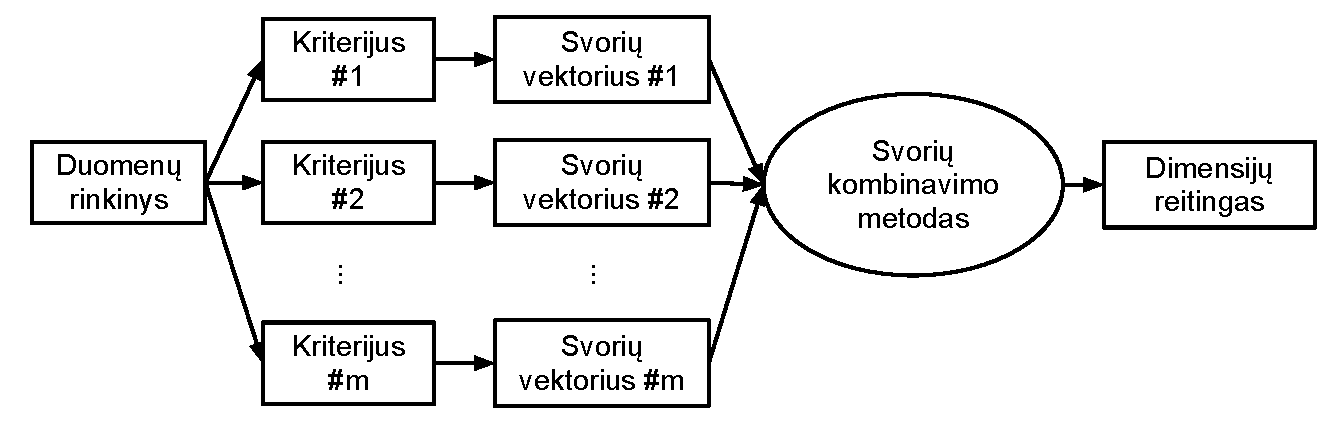
\includegraphics[width=1\textwidth]{../bachelor/images/score_based_fusion.pdf}
 \caption{Svoriais grįstas multikriterinis suliejimas.}
 \label{fig:figure4}
\end{figure}
\begin{figure}[ht]
\begin{minipage}[b]{0.5\linewidth}
\centering
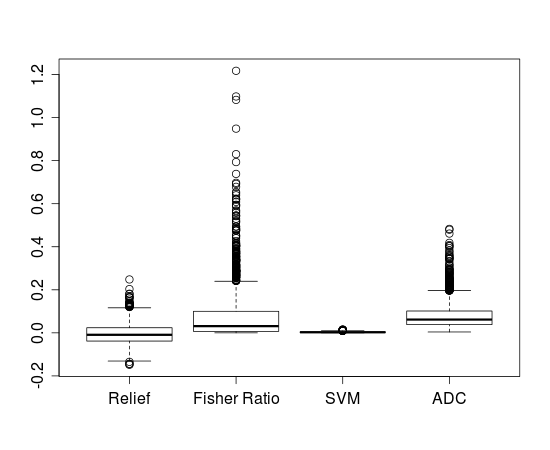
\includegraphics[width=1\textwidth]{../bachelor/images/boxplot_colon_all.png}
\caption{Pavienių matų atrinkimo metodų nenormalizuotas svorių pasiskirstymas.}
\label{fig:figure1}
\end{minipage}
\hspace{0.5cm}
\begin{minipage}[b]{0.5\linewidth}
\centering
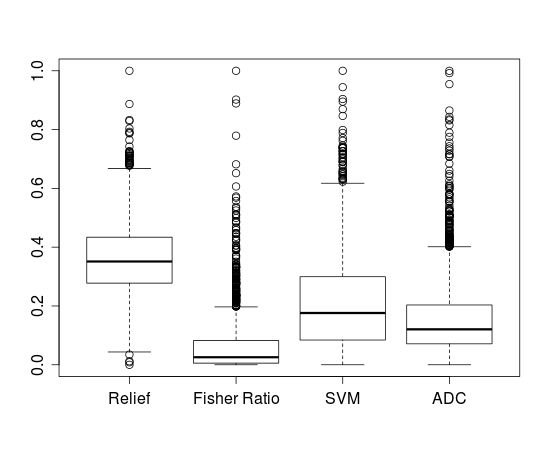
\includegraphics[width=1\textwidth]{../bachelor/images/boxplot_colon_all_normalized.png}
\caption{Pavienių matų atrinkimo metodų normalizuotas svorių pasiskirstymas.}
\label{fig:figure2}
\end{minipage}
\end{figure}

Suliejant svorius svarbu yra užtikrinti, kad svoriai, gauti naudojant
skirtingus bazinius kriterijus, būtų palyginami. Todėl svorių normalizavimas
turi būti atliekamas prieš svorių kombinavimą. Kitu
atveju matų įvertinimai bus nepalyginami. Paveikslėlyje ~\ref{fig:figure1} pav.
nenormalizuotų pavienių matų vertinimo metodų skiriasi netgi suteiktų
svorių intervalai. Paveikslėlyje ~\ref{fig:figure2} pav. matome,
kad net ir normalizavus svorius gana stipriai skiriasi svorių kvartiliai -- 
tai reikia atkreipti dėmesį interpretuojant galutinius matų vertinimo 
rezultatus. Šiame darbe svoriai yra normalizuoti intervale $[0, 1]$ pagal formulę:
\begin{equation}
 u_i'=\frac{u_i - u_{i_{min}}}{u_{i_{max}} - u_{i_{min}}}, 
\end{equation}
kur $u_i$ - matų svorių vektorius pagal $i$ kriterijų, 
$u_{i_{min}}$ - minimali $u_i$ svorių vektoriaus reikšmė,
$u_{i_{max}}$ - maksimali $u_i$ svorių vektoriaus reikšmė,
$u_i'$ - normalizuotų svorių vektorius.

Sutarties svorių vektorius $u$ yra vidurkis normalizuotų svorių vektorių:
\begin{equation}
 u = \frac{1}{m}\sum_{i=1}^m u_i',
\end{equation}
kur $m$ yra bazinių kriterijų skaičius. Reikia paminėti, kad didesnė svorio reikšmė reiškia, kad dimensija yra reikšmingesnė klasifikavimui.

\subsubsection{Reitingais grįstas multikriterinis suliejimas}

Reitingais grįsto multikriterinio suliejimo pagal reitingus metodas gauna
mėginių aibę aprašančių matų reitingą, pagal keletą bazinių matų reitingavimo kriterijų. Algoritmo pirmajame žingsnyje
keletas matų atrinkimo kriterijų grąžina matų reitingus, paskui tie reitingai yra kombinuojami į vieną bendra matų reitingą. Algoritmas yra
pavaizduotas ~\ref{fig:figure5} pav.
\begin{figure}
 \centering
 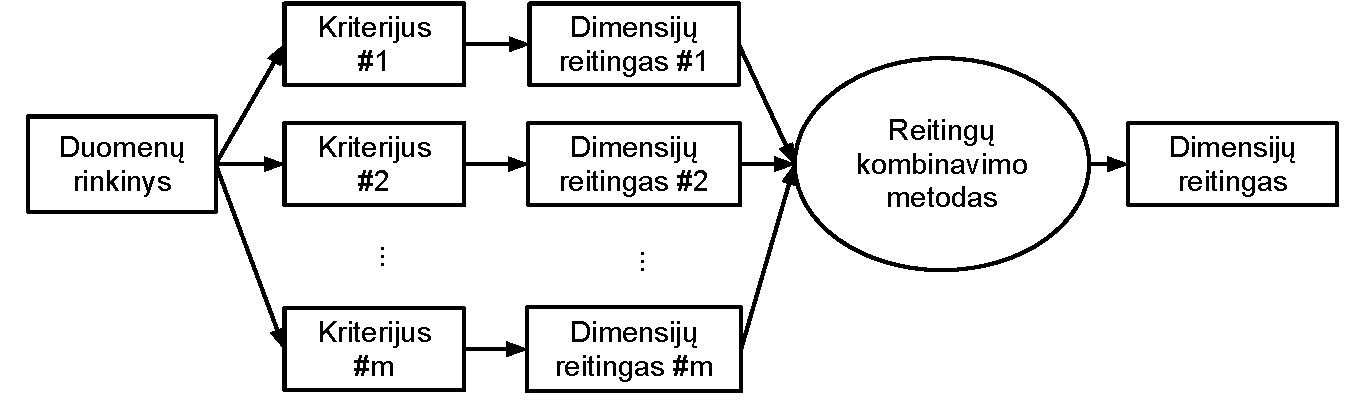
\includegraphics[width=1\textwidth]{../bachelor/images/ranking_based_fusion.pdf}
 \caption{Reitingais grįstas multikriterinis suliejimas.}
 \label{fig:figure5}
\end{figure}
Suliejimo pagal reitingus metodas nereikalauja matų atrinkimo metodų 
rezultatų normalizavimo, nes galima dimensijoms priskirtus reitingus iškart kombinuoti. Skirtingai nei suliejimo pagal svorius algoritme, baziniai 
matų atrinkimo kriterijai turi gražinti matų reitingus, o ne svorius.

Matų reitingų kombinavimui yra keletas metodų\cite{dwork2001rank}, tačiau paprastumo dėlei šiame darbe naudosiu Borda balsavimą\footnote{Dar žinomas kaip ,,Pažymių metodas``. Jis buvo pasiūlytas prancūzų matematiko ir fiziko Jean-Charles de Borda 1770 metais.} (angl. \textit{Borda count}). Tarkime, kad turime $m$ basuotojų ir $p$ kandidatų aibę. Tada Borda balsavimo metodas kiekvienam $i$-ajam balsuotojui sukuria balsų vektorių $v_i$ tokiu būdu: geriausiai įvertintam kandidatui suteikiama $p$ taškų, antrajam kandidatui $p-1$, ir t.t. Galutiniai taškai yra gaunami sudedant visų balsuotojų taškus
\begin{equation}
 v = \sum_{i=1}^m v_i,
\end{equation}
kur $v$ yra suminių taškų vektorius, o iš jo galime gauti ir galutinius matų reitingus.

\subsubsection{Svoriais ir reitingais grįstas multikriterinis suliejimas}

Svoriais ir reitingais grįsto multikriterinio suliejimo metodas nuo reitingais grįsto multikriterinio suliejimo metodo skiriasi tuo, kad kaip dar vienas reitingas yra panaudojamas svoriais grįsto multikriterinio matų atrinkimo metu gautas reitingas.
Multikriterinio matų įverčių ir pagal svorius, ir pagal reitingus metodas vyksta trimis žingsniais:
\begin{enumerate}
  \item Gauname matų reitingus pagal $m$ pavienių matų atrinkimo motodų;
  \item Suliejame matų įverčius pagal svorius, taip gauname vieną matų reitingą;
  \item Reitinguojame matus pagal visus turimus $m+1$ pavienius reitingus.
\end{enumerate} 
Algoritmas yra pavaizduotas ~\ref{fig:figure3} pav.
\begin{figure}
 \centering
 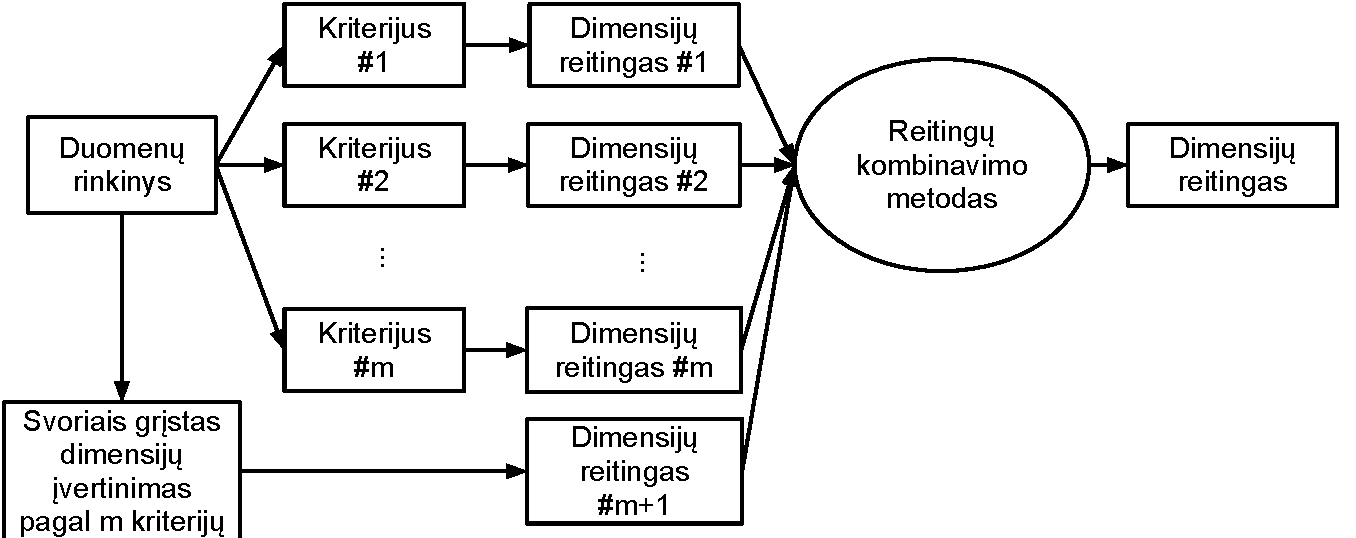
\includegraphics[width=1\textwidth]{../bachelor/images/score_and_ranking_based_fusion.pdf}
 \caption{Svoriais ir reitingais grįstas multikriterinis suliejimas.}
 \label{fig:figure3}
\end{figure}

Kadangi yra suliejami keli mažai koreliuojantys matų reitingavimo metodai, yra pasiekiamas didesnis matų atrinkimo stabilumas, kai varijuoja treniravimosi duomenų poaibis (angl. \textit{subsampling}) \cite{yang2011robust}.

\subsubsection{Multikriterinis rekursyvus matų eliminavimas}

Jei matų atrinkimo tikslas yra pagerinti klasifikavimo rezultatus, tai taikymas multikriterinių matų atrinkimo metodų nebūtinai duos pageidaujamą rezultatą, nes yra pastebėta, kad vien matų reitingavimas nebūtinai suranda geriausią matų poaibį. Tam, kad būtų surastas geriausias matų poaibis reikia kombinuoti multikriterinį matų reitingavimą su paieškos strategija. Rekursyvus matų eliminavimas yra dažnai naudojama paieškos strategija matų atrinkimui. Todėl yra kombinuojamas multikriterinis matų reitingavimas ir rekursyvus matų eliminavimas.

Multikriterinis rekursyvus matų eliminavimas\cite{yang2011robust} susideda iš dviejų dalių: keletos matų atrinkimo kriterijų suliejimo ir pagal svorius, ir 
pagal reitingus, ir rekursyvaus matų eliminavimo. Algoritmas pavaizduotas ~\ref{fig:figure6} pav.
\begin{figure}
 \centering
 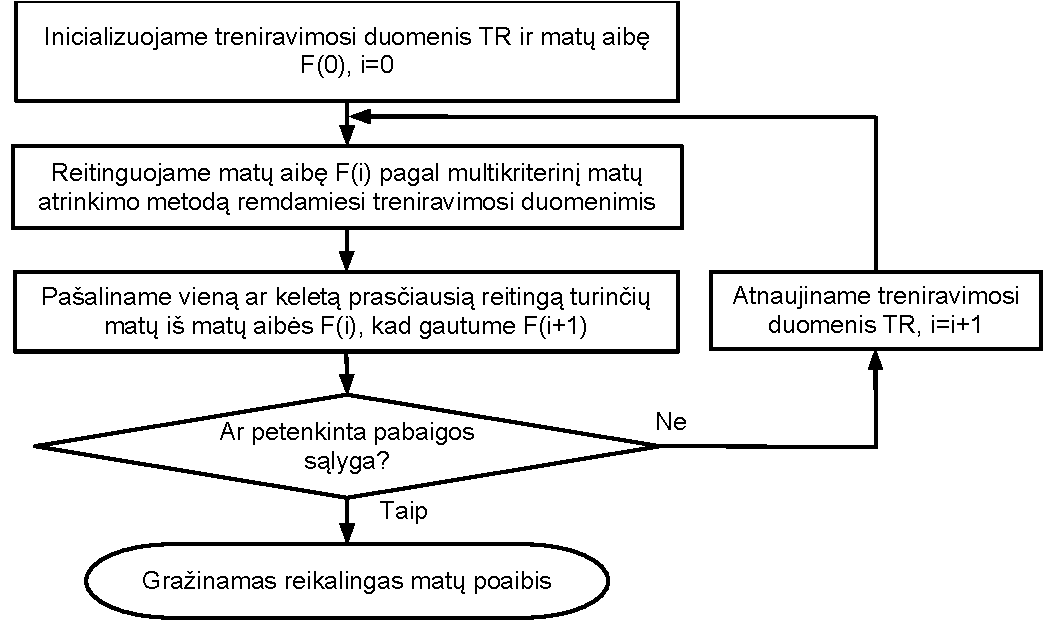
\includegraphics[width=0.8\textwidth]{../bachelor/images/mcf-rfe_procedure.pdf}
 \caption{Multikriterinio rekursyvaus matų eliminavimo algoritmas.}
 \label{fig:figure6}
\end{figure}
Standartinis rekursyvus matų eliminavimas, kai vienos iteracijos metu yra eliminuojamas vienas matas, padidina algoritmo sudėtingumą. Todėl genų ekspresijos duomenims prasmingiau yra eliminuoti keletą matų kiekvienoje iteracijoje.

Nors SVM-RFE (angl. \textit{Support Vector Machines -- Recursive Feature Elimination}) matų atrinkimo algoritmas ir yra labai populiarus, tačiau yra žinoma, kad jam trūksta stabilumo \cite{guyon2002gene}. Todėl kombinuodami didesnį stabilumą turintį multikriterinį matų atrinkimą su rekursyvaus matų eliminavimo paieškos
strategija, gauname stabilesnį matų atrinkimo algoritmą.

\subsection{Konsensuso grupėmis grįstas stabilių matų atrinkimo metodas}

Konsensuso grupėmis grįstas stabilių matų atrinkimo metodas(angl. \textit{Consensus Group Stable feature selection}, CGS), pirma, identifikuoja panašių matų grupes, antra, pagal surastas grupes transformuoja matų aibę, trečia, transformuotoje matų aibėje atlieka matų atrinkimą \cite{loscalzo2009consensus}. Schematiškai šis algoritmas pavaizduotas ~\ref{fig:figure7} pav. 
\begin{figure}
 \centering
 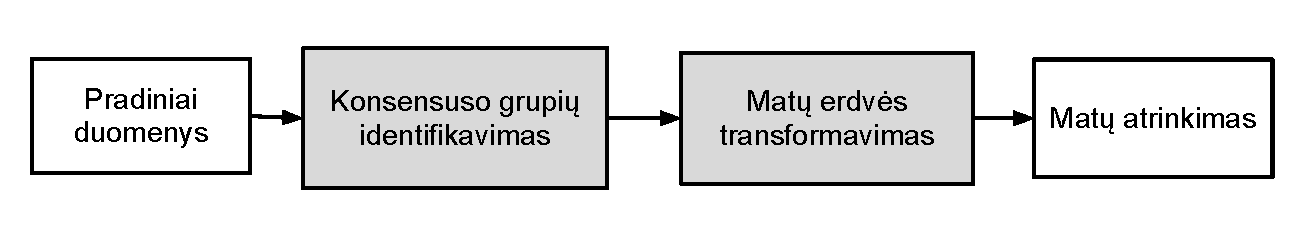
\includegraphics[width=\textwidth]{../bachelor/images/consensus_group_based_feature_selection_framework.pdf}
 \caption{Konsensuso grupėmis grįstas stabilių matų atrinkimas.}
 \label{fig:figure7}
\end{figure}

CGS metodo pagrindinė dalis yra panašių matų identifikavimas. Šio uždavinio sprendimui naudojamas \textit{Dense Group Finder} (DGF) algoritmas. DGF aprašytas algoritme nr. \ref{DGF}. CGS algoritme agal matai pagal DGF algoritmą yra sugrupuojami keletą kartų. Po pakartotinio grupavimo yra ieškoma stabilių grupių -- jei matas buvo sugrupuotas į konkrečią grupę daugiau nei pusėje grupavimų, tai matas ir priklausys tai konsensuso grupei. Matų aibės transformavimas vyksta iš kiekvienos konsensuso grupės išrenkant reprezentatyviausią matą -- konkretų matą esantį arčiausiai konsensuso grupės vidurkio. Išrinktieji reprezentatyviausieji matai ir sudaro transformuotą matų aibę. Transformuotoje matų aibėje vykdomas matų antrinkimas koriuo nors matų atrinkimo metodu $\Phi$, pavyzdžiui, \textit{Relief} matų atrinkimo metodu. 
\begin{algorithm}
\caption{DGF -- \textit{Dense Group Finder}}
\label{DGF}
 \begin{algorithmic}
 \item \textbf{Įeitis:} duomenys $D=\{x_i\}_{i=1}^n$, branduolio plotis $h$
 \item \textbf{Išeitis:} tankios matų grupės $G_1, G_1,..., G_L$
 \For{$i = 1$ \textbf{to} $n$ \do} 
  \State Inicializuojame $j=1, y_{i,j}=x_i$
  \Repeat
    \State Suskaičiuoti tankio centrą $y_{i, j+1}$ pagal (\ref{for_dgf})
  \Until{konverguoja}
  \State Nustatyti tankio centrą $y_{i,c} = y_{i,j+1}$ (Nustatyti piką $p_i$ kaip $y_{i,c}$)
  \State Sulieti piką $p_i$ su artimiausiais pikais, jei atstumai tarp jų $ < h$
 \EndFor
 \item Iš kiekvieno unikalaus piko $p_r$, pridėkime $x_i$ į $G_r$, jei $||p_r - x_i|| < h$
 \end{algorithmic}
\end{algorithm}

\begin{equation}
\label{for_dgf}
  y_{i, j+1}=\frac{\sum_{i=1}^{n} x_i K(\frac{y_j - x_i}{h})}{\sum_{i=1}^{n} K(\frac{y_j - x_i}{h})} j=1,2,...
\end{equation}
kur $K(x)$ -- \textit{kernel} funkcija, $h$ -- \textit{kernel} plotis, $y$ -- tankio centras.

\begin{algorithm}
 \caption{Konsensuso grupėmis grįstas stabilių matų atrinkimas}
 \label{CGS}
 \begin{algorithmic}
   \item \textbf{Įeitis:} mėginių aibė $D$, iteracijų skaičius $t$, matų atrinkimo metodas $\Phi$\
   \item \textbf{Išeitis:} atrinktos konsensuso matų grupės $CG_1, CG_1,..., CG_k$
   \item // Konsensuso grupių identifikavimas
   \For{$i = 1$ \textbf{to} $n$ \do}
    \State Parinkti mėginių  poaibį $D_i$ iš $D$
    \State Gauti panašių matų grupes pagal $DGF(D_i, h)$
   \EndFor
   \For{kiekvienai matų porai $X_i$ ir $X_j \in D$}
    \State Nustatyti $W_{i,j}=$ dažnis, kai $X_i$ ir $X_j$ yra toje pačioje grupėje $/t$
   \EndFor
   \item Sudaryti konsensuso grupes $CG_1, CG_1,..., CG_L$ atliekant hierarchinį klasterizavimą visiems matams pagal $W_{i, j}$
   \item //Matų atrinkimas grįstas konsensuso grupėmis
   \For{$i = 1$ \textbf{to} $l$ \do}
    \State Parinkti reprezentatyvų matą $X_i$ iš $CG_i$
    \State Įvertinti mato informatyvumą $\Phi(X_i)$
   \EndFor
   \item Reitinguoti konsensuso grupes $CG_1, CG_1,..., CG_L$ pagal $\Phi(X_i)$
   \item Pasirinkti $k$ matų, turinčių geriausią reitingą  
 \end{algorithmic}
\end{algorithm}

\subsection{Suprogramuotų matų atrinkimo algoritmų palyginimas}

Matų atrinkimo metodus palyginau trim aspektais: darbo laiko, klasifikavimo pagal atrinktus matus tikslumo, bei matų atrinkimo stabilumo. Toliau aprašysiu eksperimentuose gautus rezultatus atskirai.
\subsubsection{Matų atrinkimo metodų darbo laikas}

Matų atrinkimo metodų darbo laikas buvo palygintas naudojant vieną biomedicininių duomenų rinkinį - AltarA \cite{altara}. Skaičiavimai buvo atlikti kompiuteryje naudojant vieną procesoriaus branduolį veikiantį 2.66 GHz, bei 2 GB RAM atminties. ~\ref{fig:visu_laikas} pav. ir ~\ref{fig:cgs_laikas} pav. pavaizduota matų atrinkimo metodo darbo laiko priklausomybė nuo mėginius apibūdinančių matų skaičiaus. 
\begin{figure}[hq]
\begin{minipage}[b]{0.5\linewidth}
\centering
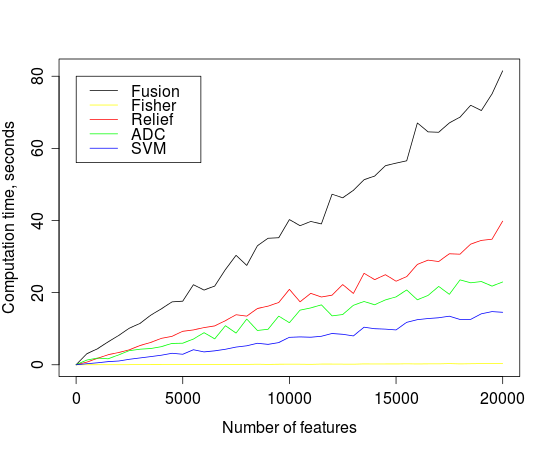
\includegraphics[width=1\textwidth]{images/all_performance.png}
 \caption{Pagrindini matų atrinkimo metodų darbo laikas.}
 \label{fig:visu_laikas}
\end{minipage}
\hspace{0.5cm}
\begin{minipage}[b]{0.5\linewidth}
\centering
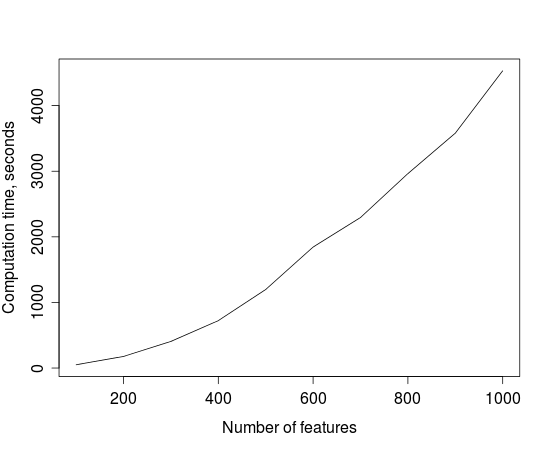
\includegraphics[width=1\textwidth]{images/cgs_performance.png}
 \caption{Konsensuso grupėmis grįsto matų atrinkimo metodo darbo laikas.}
 \label{fig:cgs_laikas}
\end{minipage}
\end{figure}
Matų atrinkimo metodų darbo laikas yra atvaizduotas dviem grafikais, nes atliekant eksperimentų rezultatai parodė, kad CGS matų atrinkimo metodas yra apie 1000 kartų lėtesnis už kitus suprogramuotus matų atrinkimo metodus, todėl viename grafike neįmanoma atvaizduoti visų turimų matų atrinkimo metodų. Pagal ~\ref{fig:visu_laikas} pav. galime daryti išvadą, kad sparčiausias matų atrinkimo metodas yra \textit{Fisher} įvertis. Pagal gautus matų darbo laiko priklausomybės nuo matų kiekio grafikus galime daryti išvadą, kad CGS algoritmas daugiamačių duomenų matų atrinkimui nėra tinkamas, nes darbo laikas yra per ilgas.

\subsubsection{Klasifikavimo pagal atrinktus matus tikslumas}

Matų atrinkimo metodų įtaką klasifikavimo klasifikavimo tikslumui buvo matuojama naudojant tris biomedicininių duomenų rinkinius: Gaubtinės žarnos auglio (angl. Colon) \cite{alon1999broad}, Centrinės nervų sistemos (CNS) \cite{pomeroy2002prediction}, prostatos \cite{singh2002gene}. Klasifikavimui buvo naudojami tiesiniai atraminių vektorių klasifikatoriai (SVM) \cite{vapnik2000nature}, su parametru $C=0.01$, kurį nustačiau  empiriškai. Keičiant parametrus keičiasi ir klasifikavimo tikslumas. Klasifikatoriui apmokyti buvo naudojama 90\% atsitiktinai parinktų mėginių iš duomenų rinkinio. Likusiais 10\% mėginių buvo testuojamas klasifikatorius. Klasifikatorius buvo testuojamas po 300 kartų su įvairiu matų skaičiumi: nuo 10 iki 500. Klasifikavimo tikslumas pavaizduotas dviejų tipų grafikais: vidutinio klaidų procento priklausomybės nuo atrinktų dimensijų skaičiaus, bei ROC kreivėmis, kurios buvo gautos pagal duomenis gautus klasifikuojant su tiek atrinktų dimensijų su kiek klasifikavimo tikslumas buvo pats geriausias \cite{green1966signal}.
\begin{figure}[H]
\begin{minipage}[b]{0.5\linewidth}
\centering
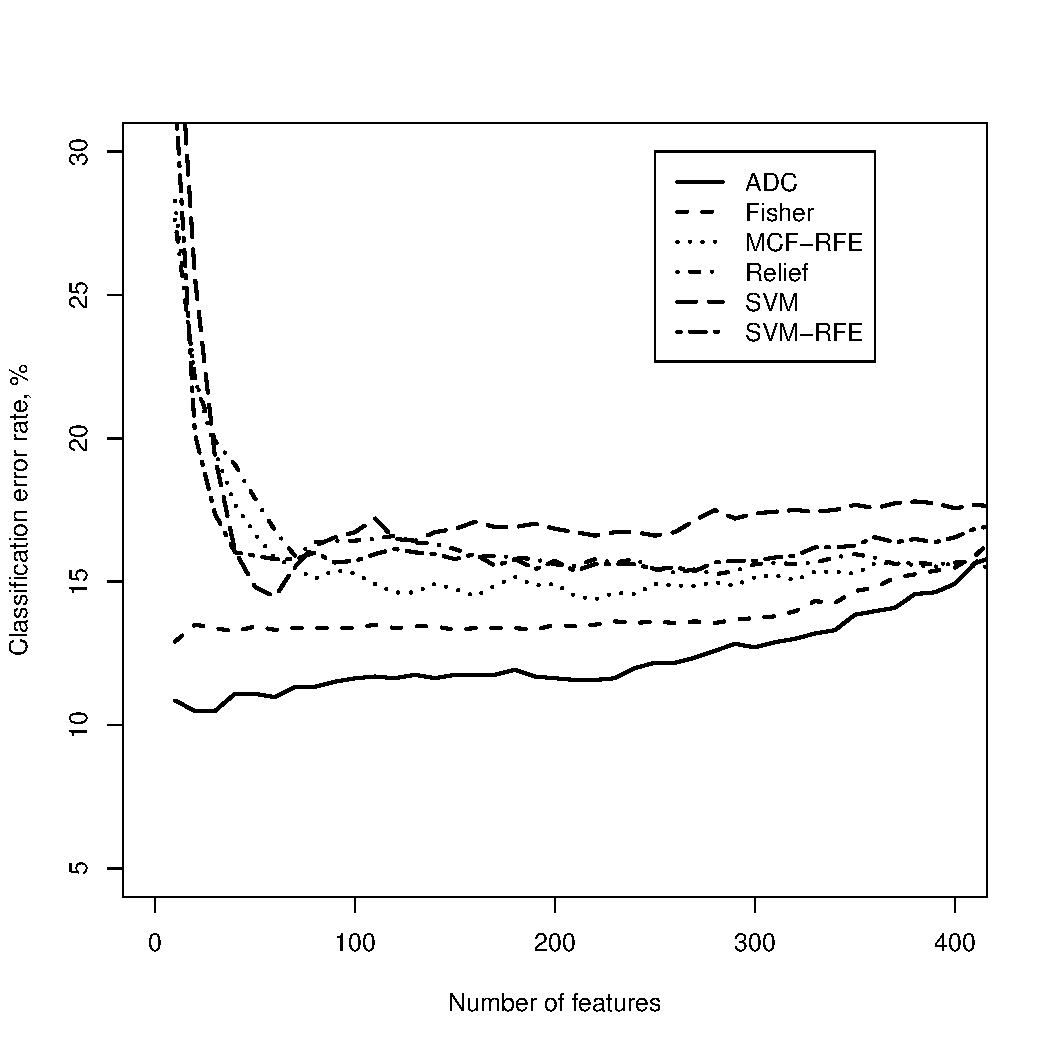
\includegraphics[width=.9\textwidth]{../bachelor/images/nncolon_classification.pdf}
\caption{Gaubtinės žarnos auglio meginių klasifikatorių tikslumas.}
\label{fig:class_colon}
\end{minipage}
\hspace{0.2cm}
\begin{minipage}[b]{0.5\linewidth}
\centering
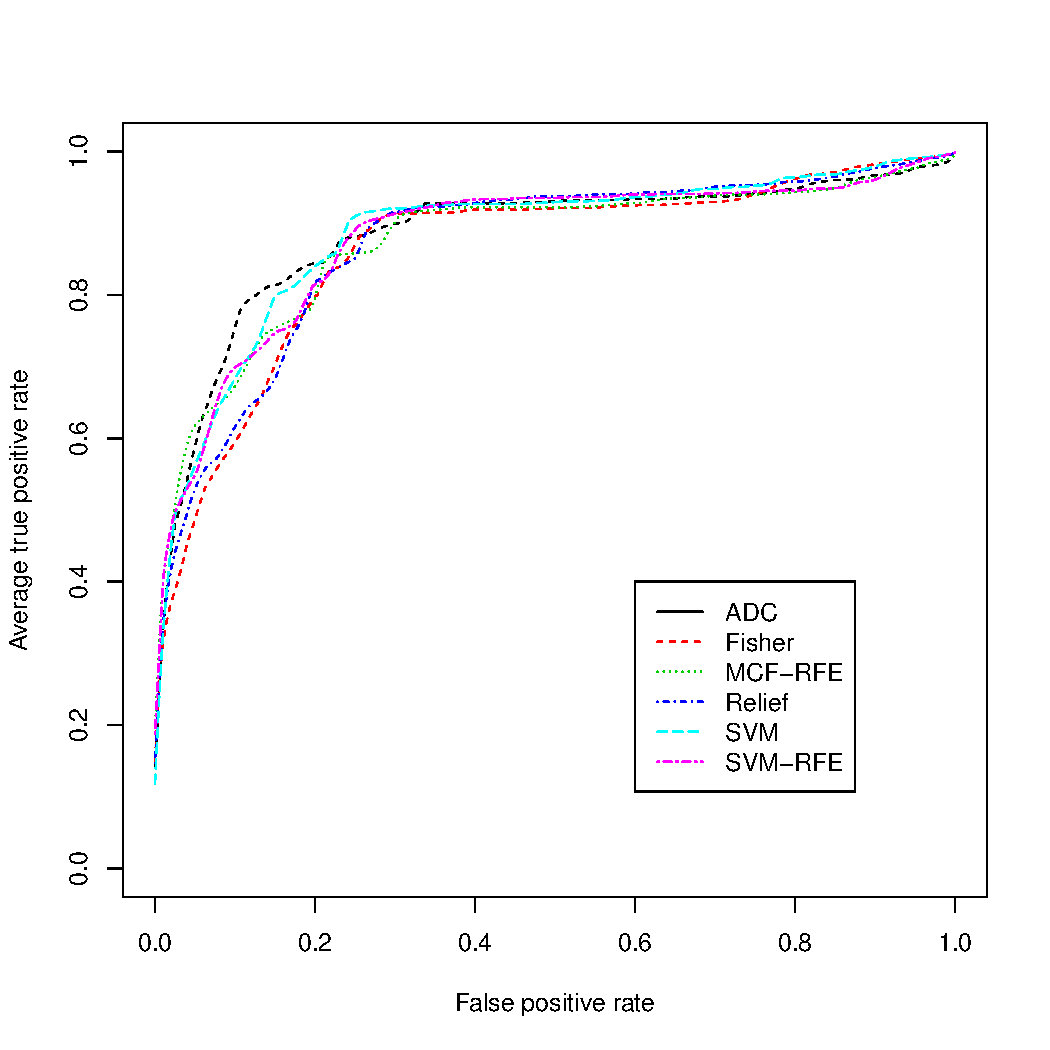
\includegraphics[width=.85\textwidth]{../bachelor/images/nncolon_roc.pdf}
\caption{Gaubtinės žarnos auglio mėginių klasifikatorių ROC kreivės.}
\label{fig:roc_colon}
\end{minipage}
\hspace{0.2cm}
\begin{minipage}[b]{0.5\linewidth}
\centering
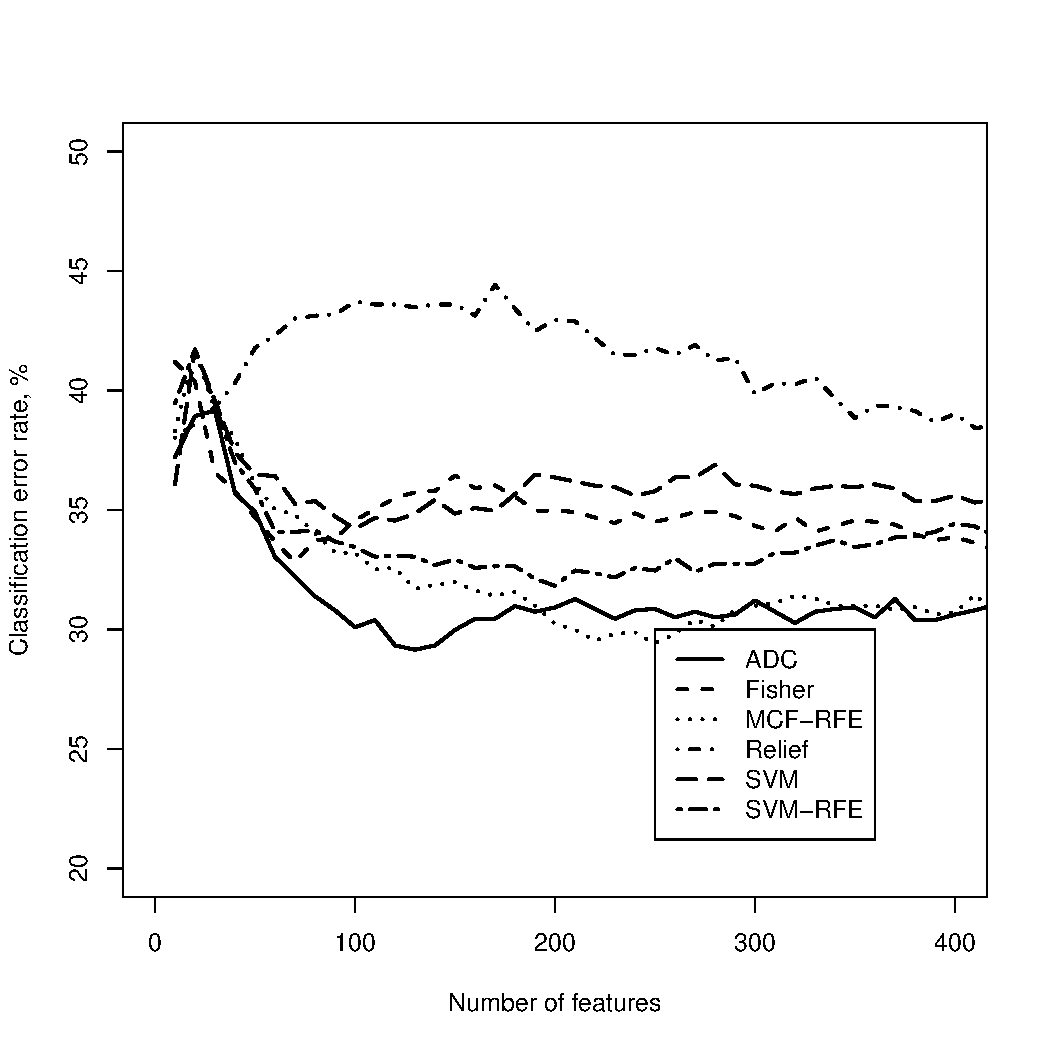
\includegraphics[width=.85\textwidth]{../bachelor/images/nncns_classification.pdf}
\caption{Centrinės nervų sistemos meginių klasifikatorių tikslumas.}
\label{fig:class_cns}
\end{minipage}
\hspace{0.2cm}
\begin{minipage}[b]{0.5\linewidth}
\centering
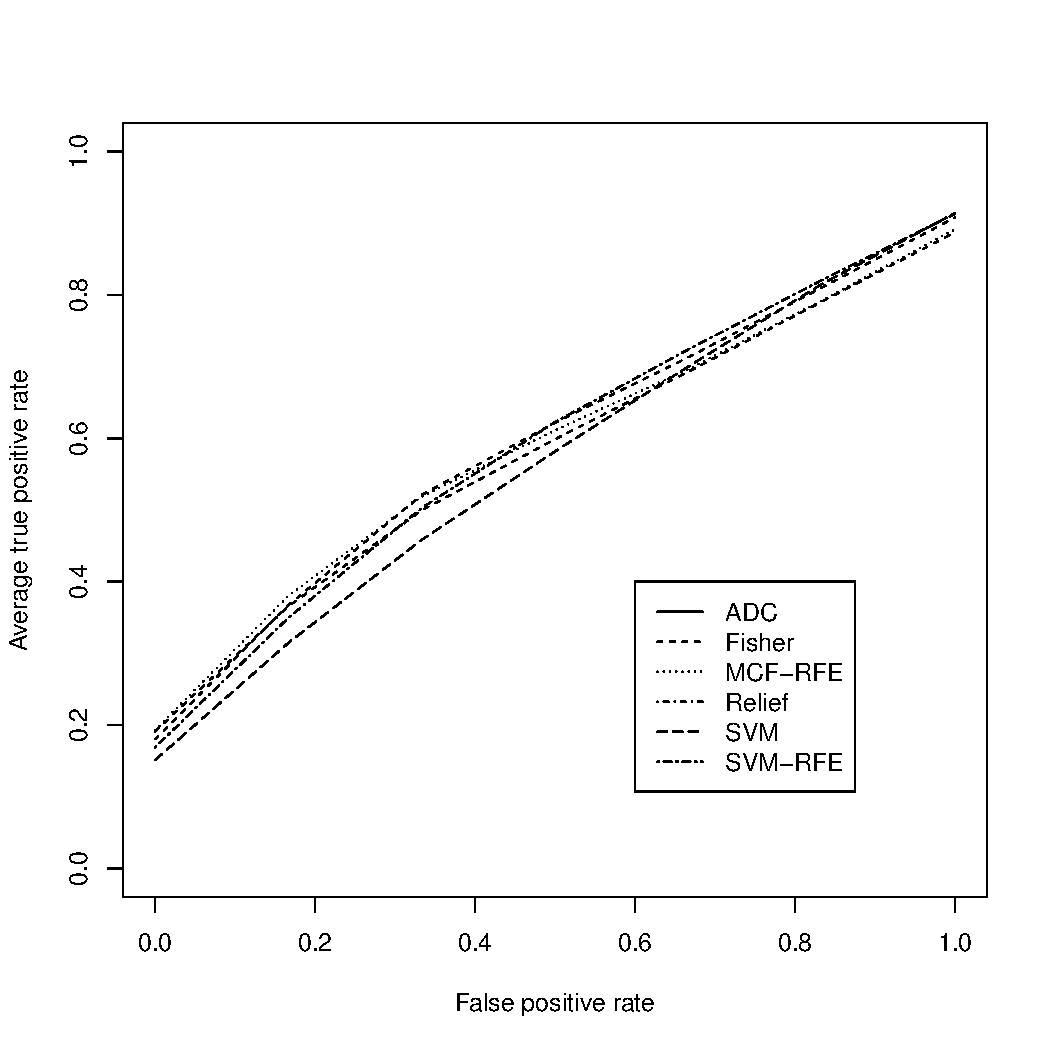
\includegraphics[width=.85\textwidth]{../bachelor/images/nncns_roc.pdf}
\caption{Centrinės nervų sistemos mėginių klasifikatorių ROC kreivės.}
\label{fig:roc_cns}
\end{minipage}
\hspace{0.2cm}
\begin{minipage}[b]{0.5\linewidth}
\centering
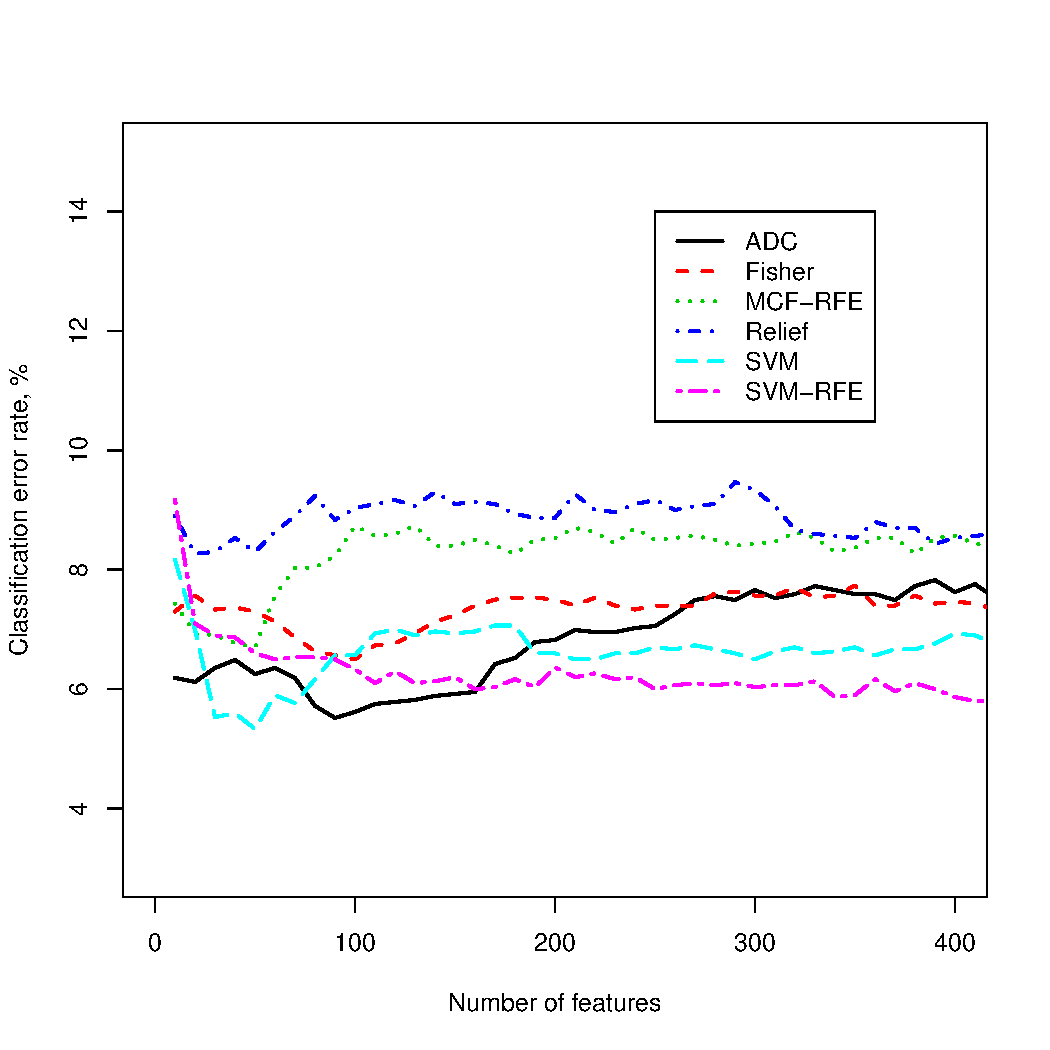
\includegraphics[width=.85\textwidth]{../bachelor/images/prostate_classification.pdf}
\caption{Prostatos meginių klasifikatorių tikslumas.}
\label{fig:class_prostate}
\end{minipage}
\hspace{0.2cm}
\begin{minipage}[b]{0.5\linewidth}
\centering
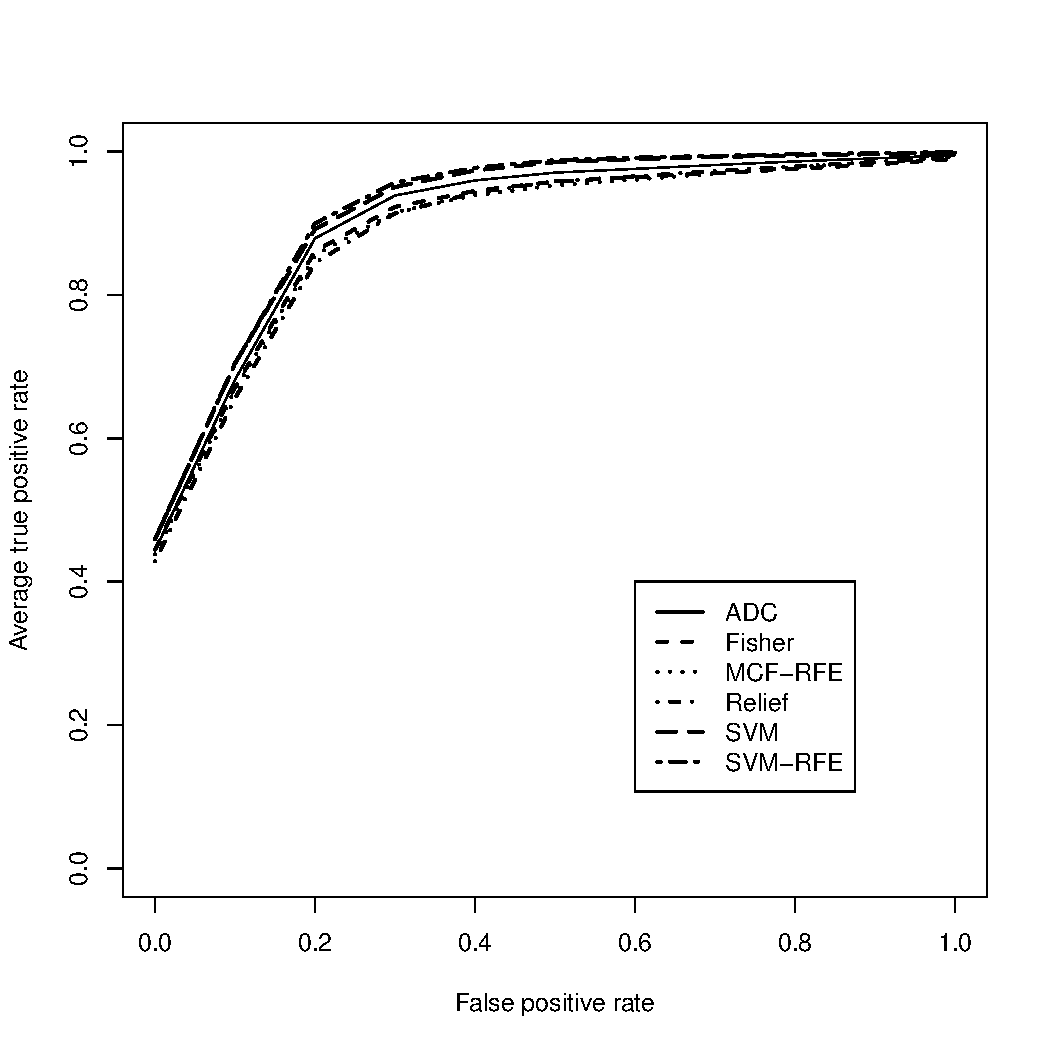
\includegraphics[width=.85\textwidth]{../bachelor/images/prostate_roc.pdf}
\caption{Prostatos mėginių klasifikatorių ROC kreivės.}
\label{fig:roc_prostate}
\end{minipage}
\end{figure}
~\ref{fig:class_colon} pav. matome, kad gaubtinės žarnos auglio duomenų rinkinio matus geriausiai atrenka ADC metodas. Tik šiek tiek prasčiau pasirodo \textit{Fisher} įvertis. Blogiausiai su gaubtinės žarnos auglio mėginiais susidoroja absoliučių svorių SVM matų atrinkimo metodas.

% % \begin{figure}[hw]
% % \begin{minipage}[b]{0.5\linewidth}
% % \centering
% % 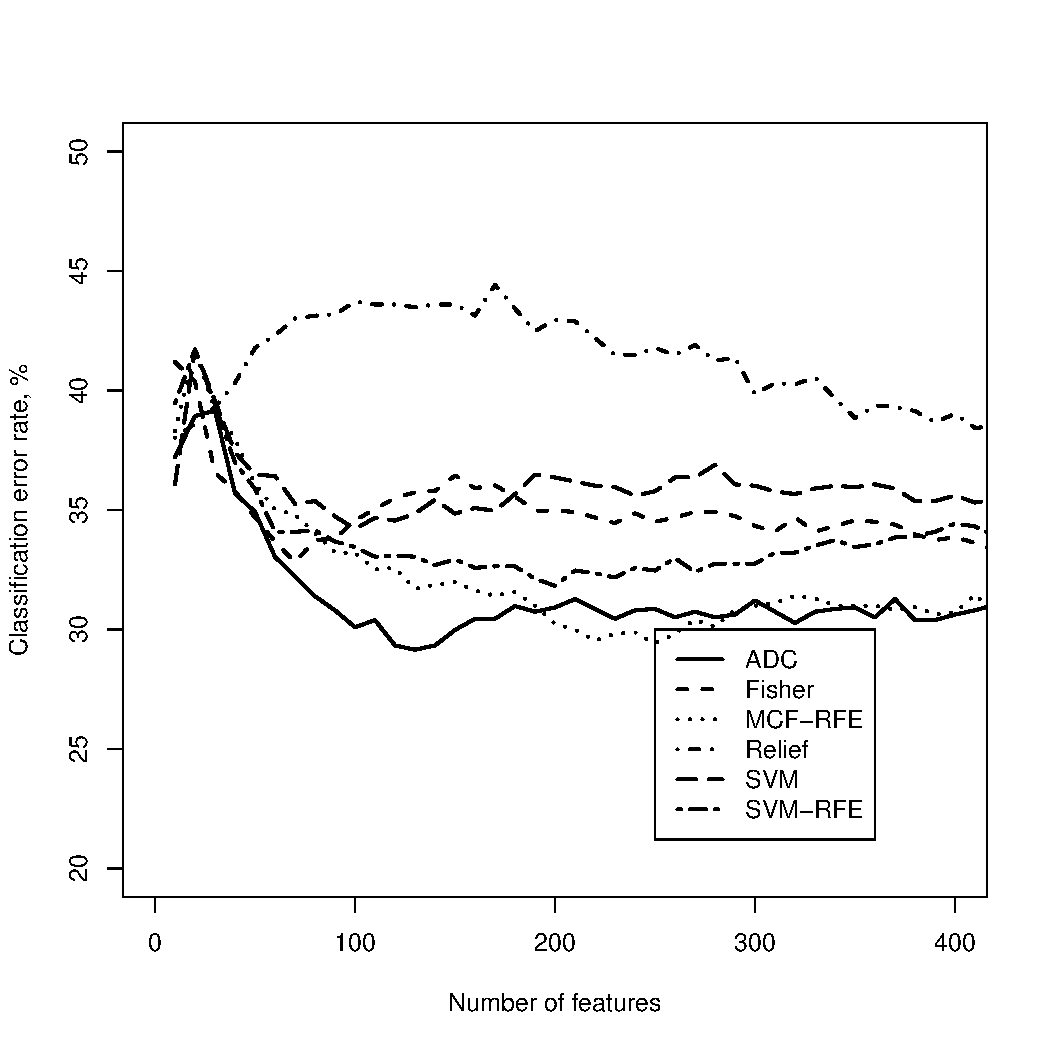
\includegraphics[width=1\textwidth]{../bachelor/images/nncns_classification.pdf}
% % \caption{Centrinės nervų sistemos meginių klasifikatorių tikslumas.}
% % \label{fig:class_cns}
% % \end{minipage}
% % \hspace{0.5cm}
% % \begin{minipage}[b]{0.5\linewidth}
% % \centering
% % 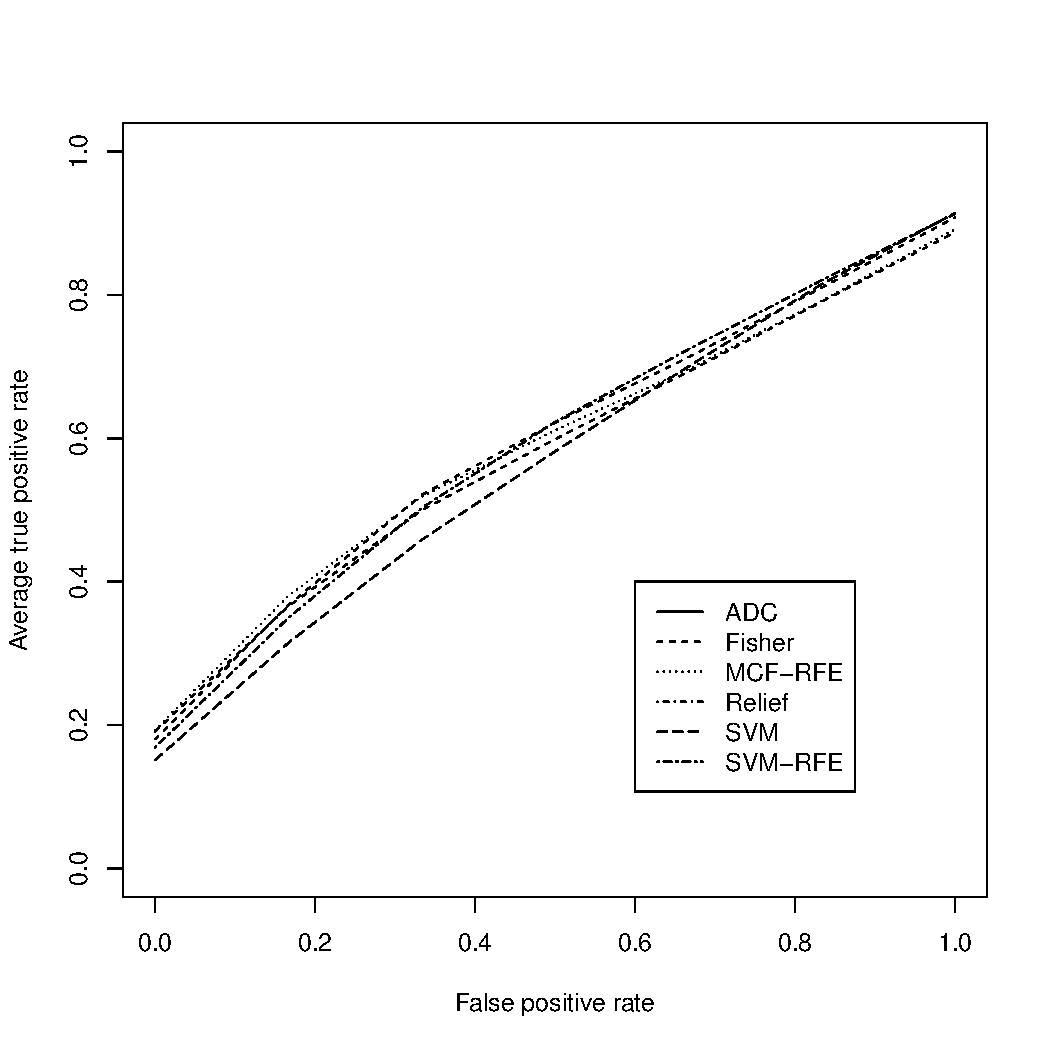
\includegraphics[width=1\textwidth]{../bachelor/images/nncns_roc.pdf}
% % \caption{Centrinės nervų sistemos mėginių klasifikatorių ROC kreivės.}
% % \label{fig:roc_cns}
% % \end{minipage}
% % \end{figure}
Centrinės nervų sistemos duomenų rinkinys yra sunkiai klasifikuojamas, nes vidutinis klaidų skaičius yra apie 35\%, kai, pvz. gautinės žarnos auglio duomenų rinkinio vidutinis klaidų skaičius yra tik 15\%. ~\ref{fig:class_cns} pav. matome, kad šiam duomenų rinkiniui vidutiniškai geriausiai matus atrenka ADC ir multikriterinio rekursyvaus dimensijų eliminavimo metodai. Prasčiausiai pasirodo \textit{Relief} metodas.

% \begin{figure}[h]
% \begin{minipage}[b]{0.5\linewidth}
% \centering
% 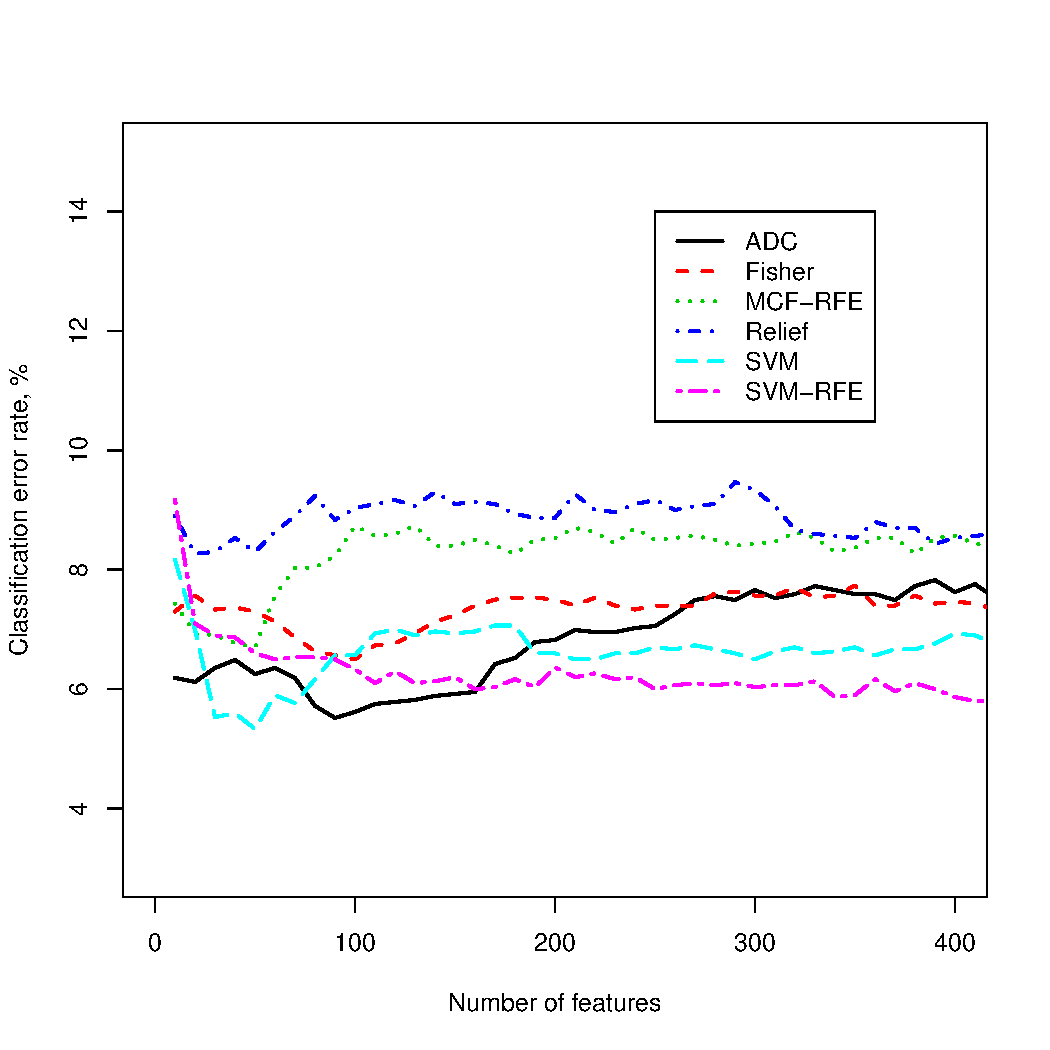
\includegraphics[width=1\textwidth]{../bachelor/images/prostate_classification.pdf}
% \caption{Prostatos meginių klasifikatorių tikslumas.}
% \label{fig:class_prostate}
% \end{minipage}
% \hspace{0.5cm}
% \begin{minipage}[b]{0.5\linewidth}
% \centering
% 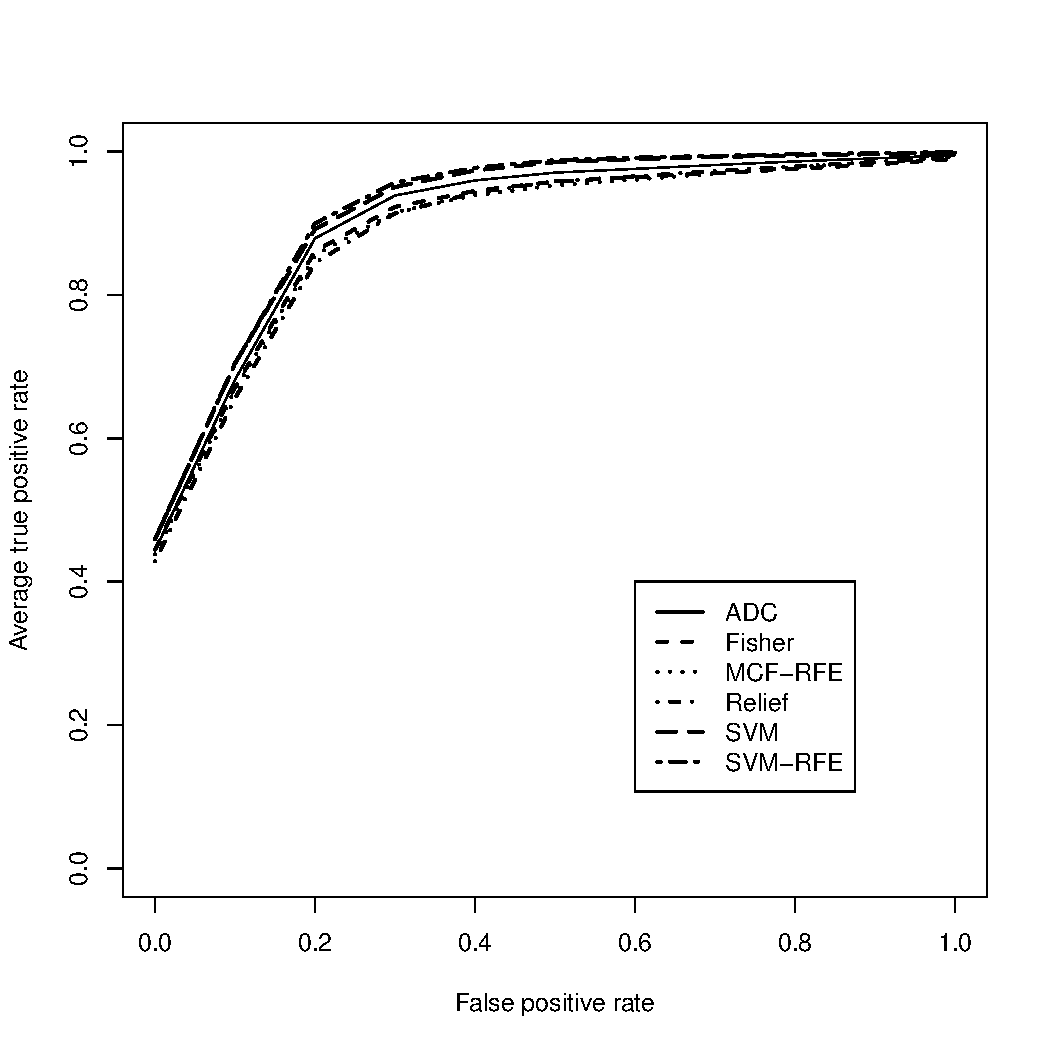
\includegraphics[width=1\textwidth]{../bachelor/images/prostate_roc.pdf}
% \caption{Prostatos mėginių klasifikatorių ROC kreivės.}
% \label{fig:roc_prostate}
% \end{minipage}
% \end{figure}
~\ref{fig:class_prostate} pav. matome, kad prostatos duomenų rinkinio matus klasifikavimui geriausiai atrenka ADC absoliučių svorių SVM metodas. Prasčiausiai matus atrenka \textit{Relief}.

Apibendrindamas gautus klasifikavimo tikslumo matavimo rezultatus, galiu teigti, kad nėra vieno absoliučiai geriausio matų atrinkimo metodo. Reikia eksperimentuoti, kad būtų rastas konkrečiai problemai geriausiai tinkantis matų atrinkimo metodas. Tačiau rezultatai parodė, kad matų atrinkimas svariai prisideda prie geresnio klasifikatoriaus sukūrimo.

\subsubsection{Matų atrinkimo stabilumas}

Matų atrinkimo stabilumas buvo tiriamas naudojant tuos pačius biomedicininių duomenų rinkinius kaip ir tiriant klasifikavimo pagal atrinktus matus tikslumą. Matų atrinkimo stabilumas buvo matuojamas pagal \textit{Kuncheva} ir \textit{Jaccard} indeksus. Stabilumas pats savaime nėra svarbus, jis turi būti matuojamas atsižvelgiant į klasifikavimo tikslumą. Todėl šio skyrelio grafikus reikia nagrinėti atsižvelgiant į skyrelio, kuriame buvo nagrinėtas klasifikavimo pagal atrinktus matus tikslumas.

\begin{figure}[H]
\begin{minipage}[b]{0.5\linewidth}
\centering
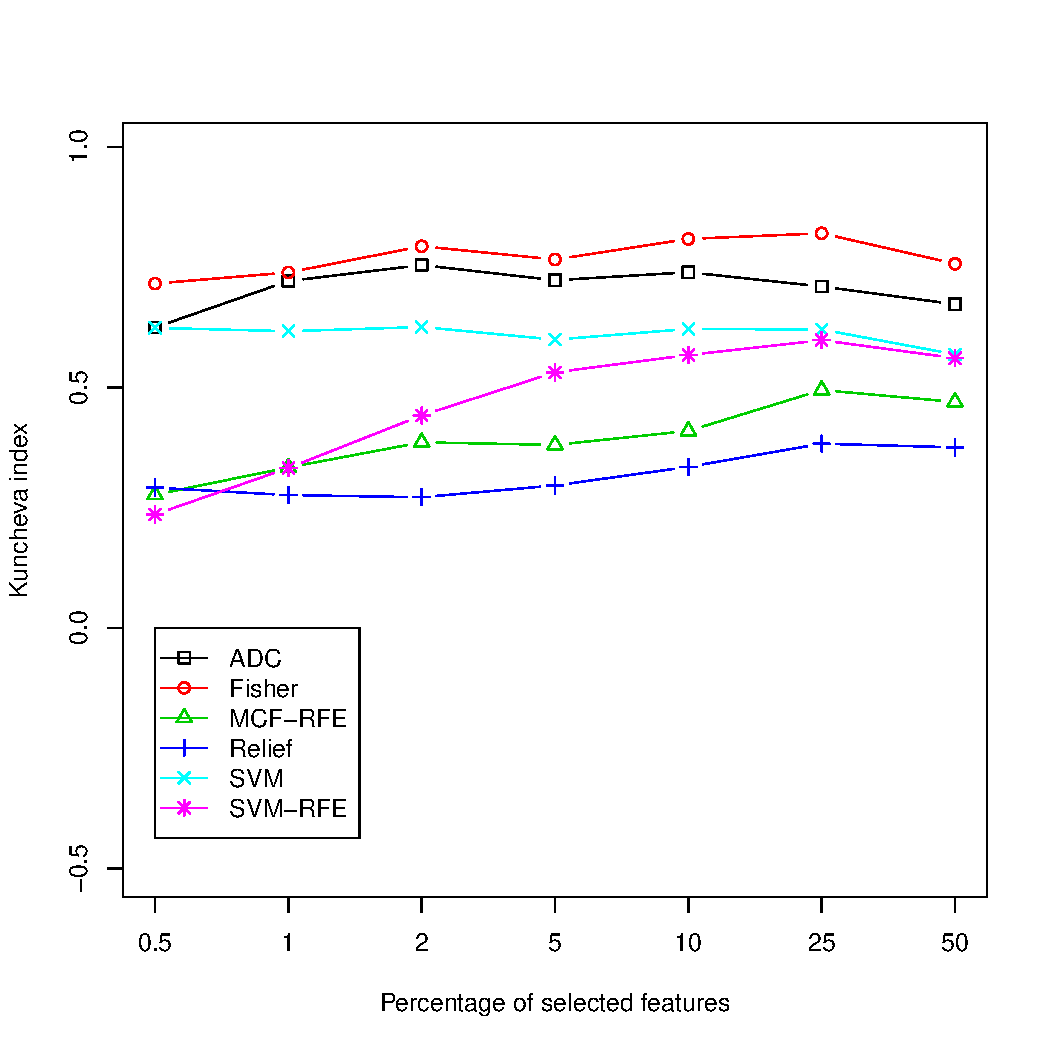
\includegraphics[width=.85\textwidth]{../bachelor/images/nncolon_robustness_kuncheva.pdf}
\caption{Matų atrinkimo gaubtinės žarnos auglio mėginiams stabilumo grafikas pagal Kuncheva indeksą.}
\label{fig:robk_colon}
\end{minipage}
\hspace{0.2cm}
\begin{minipage}[b]{0.5\linewidth}
\centering
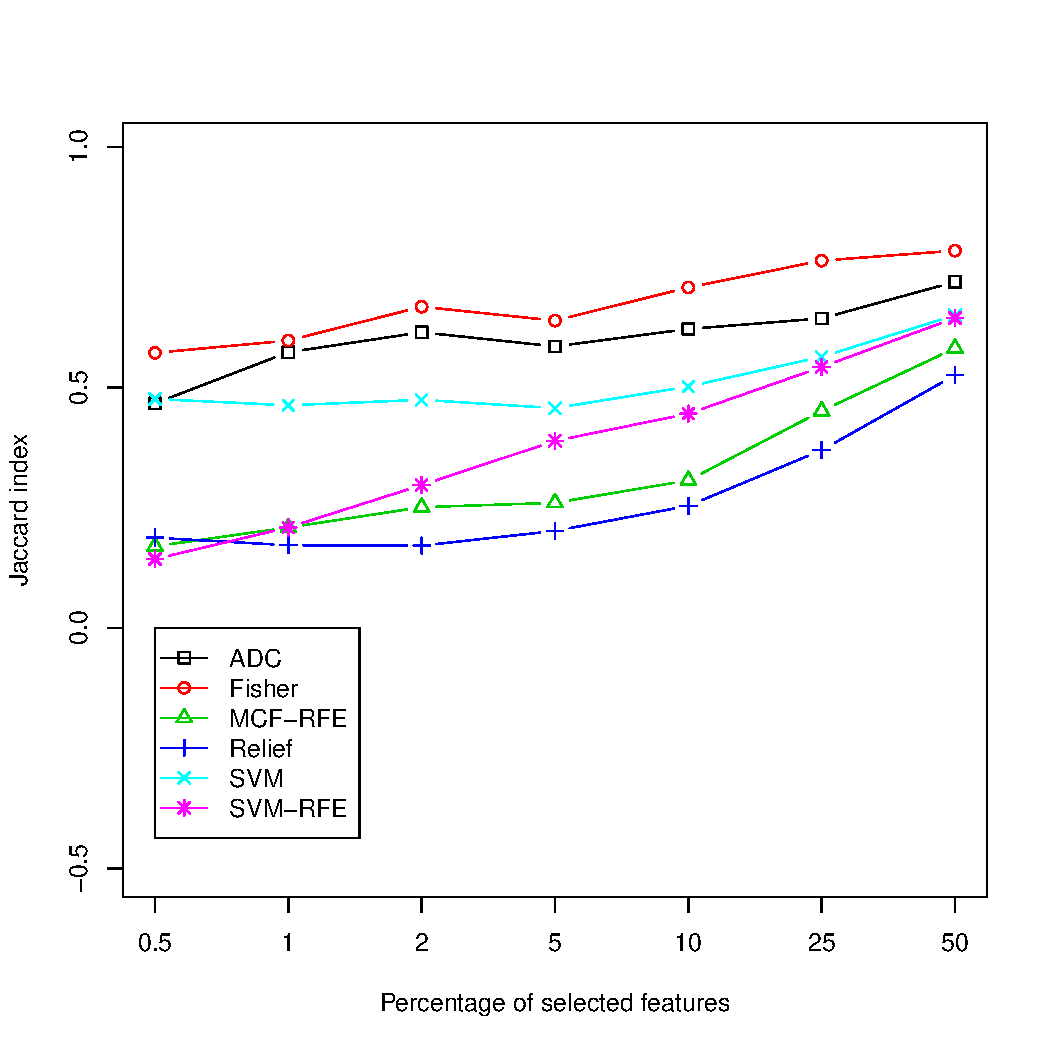
\includegraphics[width=.85\textwidth]{../bachelor/images/nncolon_robustness_jaccard.pdf}
\caption{Matų atrinkimo gaubtinės žarnos auglio mėginiams stabilumo grafikas pagal Jaccard indeksą.}
\label{fig:robj_colon}
\end{minipage}
\hspace{0.2cm}
\begin{minipage}[b]{0.5\linewidth}
\centering
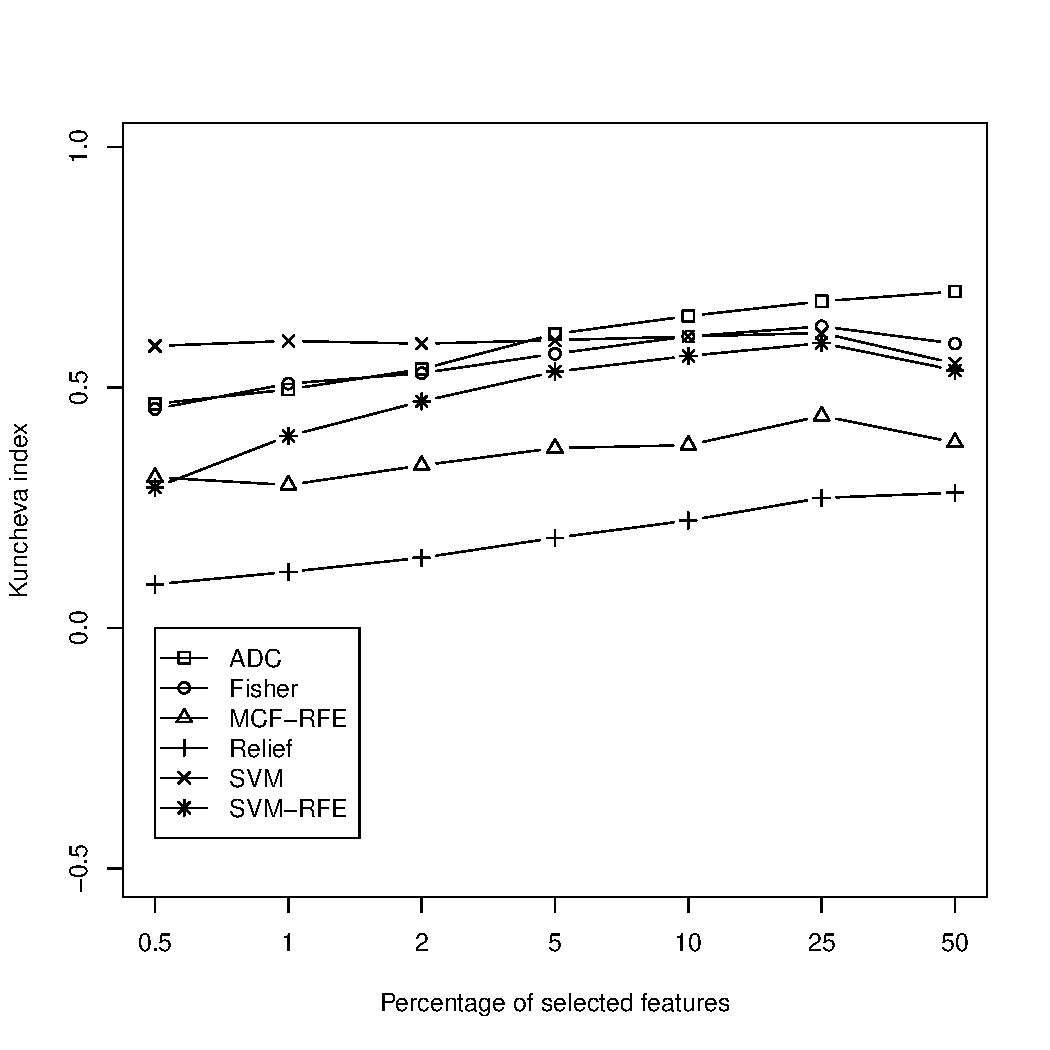
\includegraphics[width=.85\textwidth]{../bachelor/images/nncns_robustness_kuncheva.pdf}
\caption{Matų atrinkimo CNS mėginiams stabilumo grafikas pagal Kuncheva indeksą.}
\label{fig:robk_cns}
\end{minipage}
\hspace{0.2cm}
\begin{minipage}[b]{0.5\linewidth}
\centering
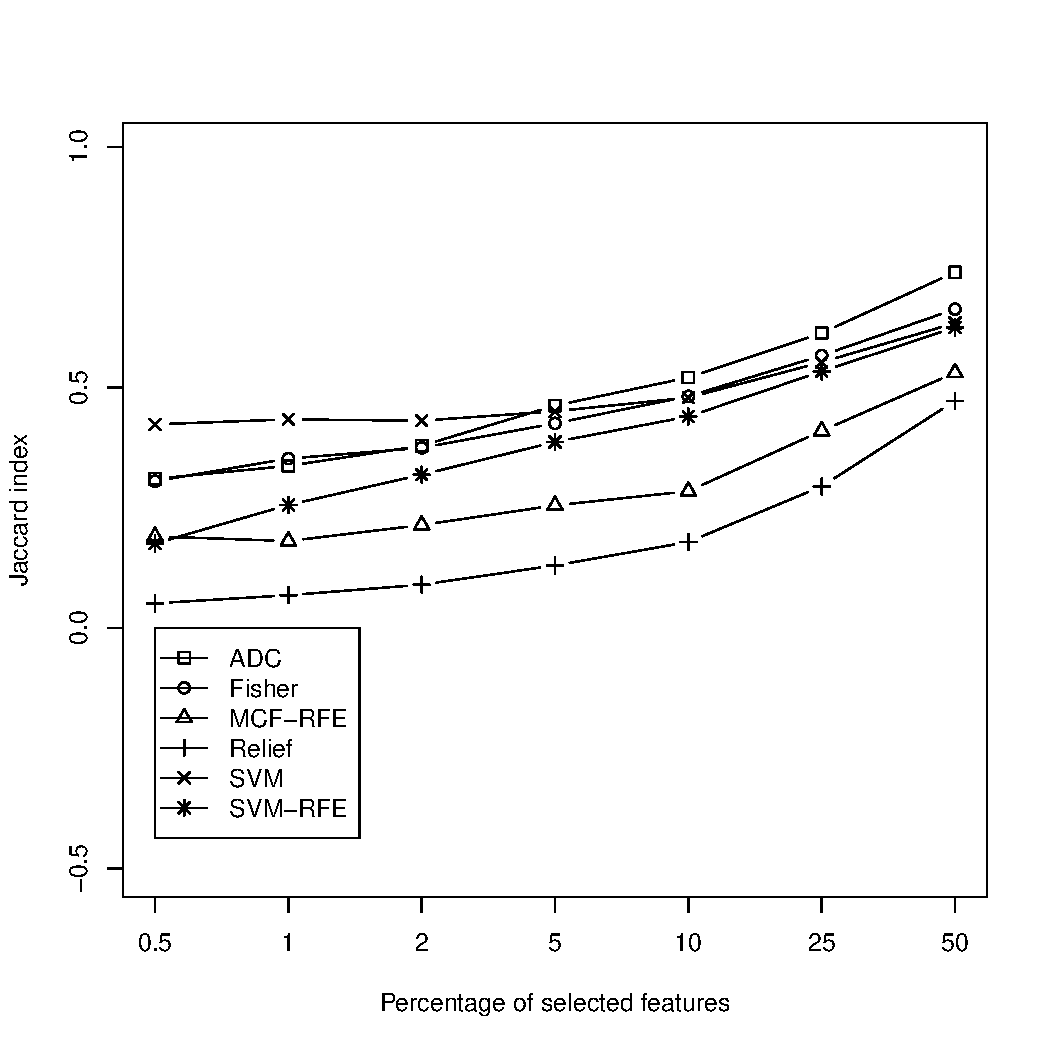
\includegraphics[width=.85\textwidth]{../bachelor/images/nncns_robustness_jaccard.pdf}
\caption{Matų atrinkimo CNS mėginiams stabilumo grafikas pagal Jaccard indeksą.}
\label{fig:robj_cns}
\end{minipage}
\hspace{0.2cm}
\begin{minipage}[b]{0.5\linewidth}
\centering
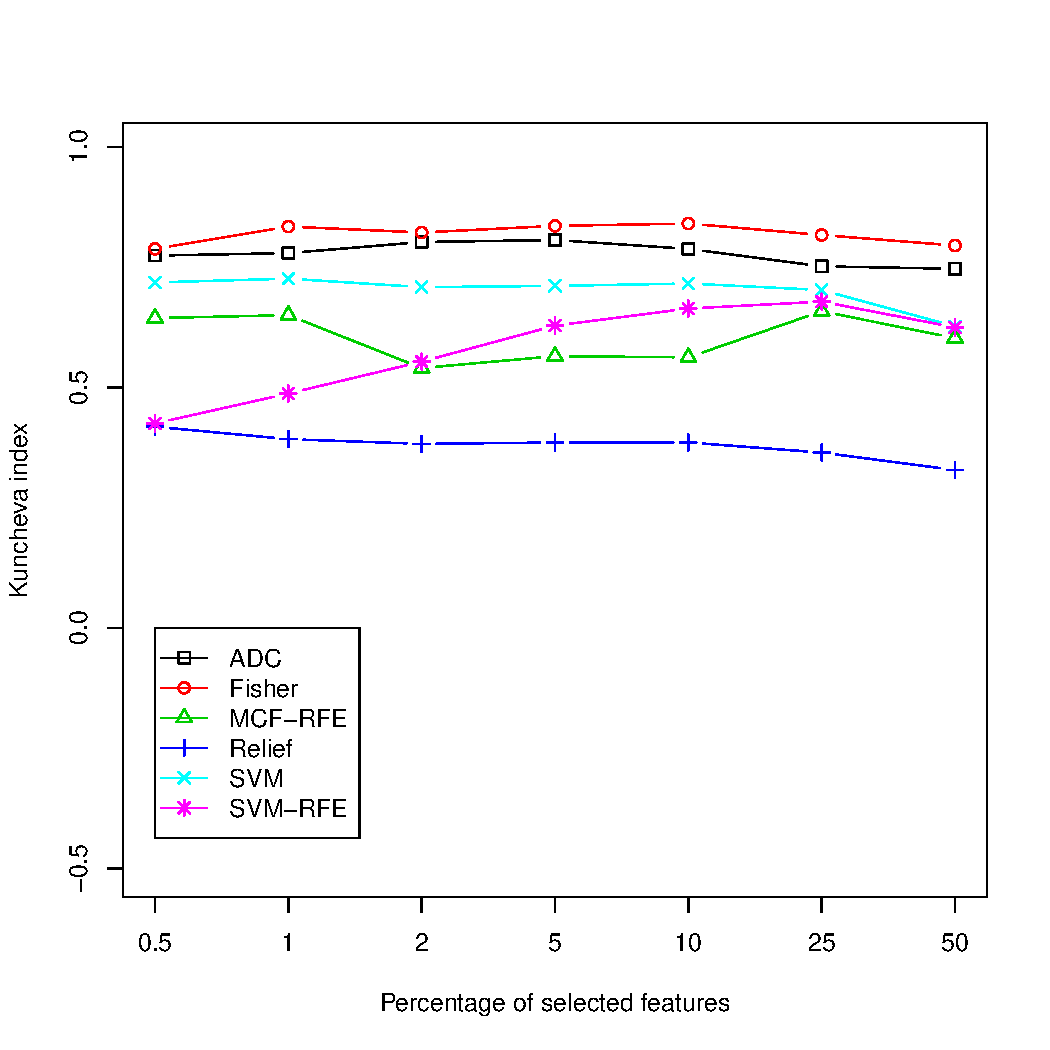
\includegraphics[width=.85\textwidth]{../bachelor/images/prostate_robustness_kuncheva.pdf}
\caption{Matų atrinkimo prostatos mėginiams stabilumo grafikas pagal Kuncheva indeksą.}
\label{fig:robk_prostate}
\end{minipage}
\hspace{0.2cm}
\begin{minipage}[b]{0.5\linewidth}
\centering
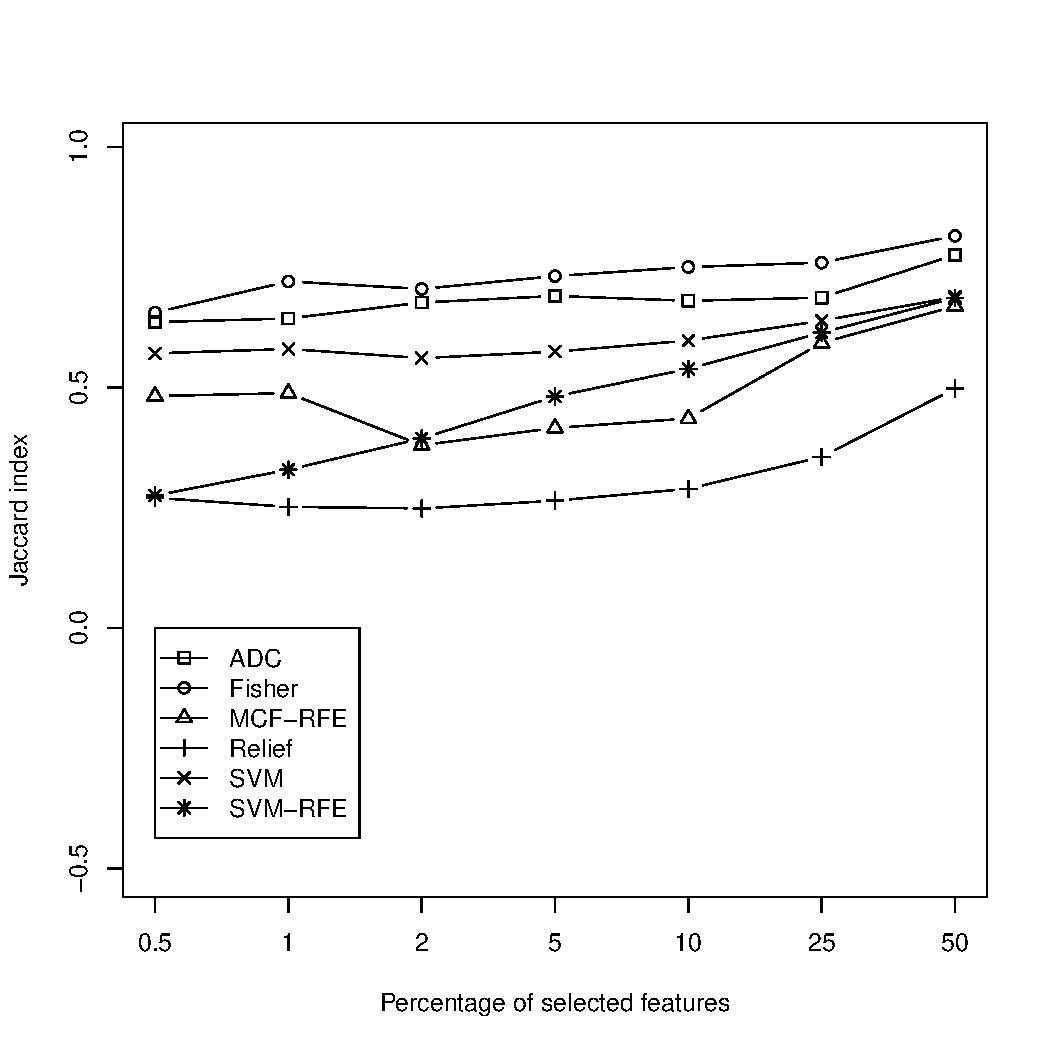
\includegraphics[width=.85\textwidth]{../bachelor/images/prostate_robustness_jaccard.pdf}
\caption{Matų atrinkimo prostatos mėginiams stabilumo grafikas pagal Jaccard indeksą.}
\label{fig:robj_prostate}
\end{minipage}
\end{figure}
Pagal ~\ref{fig:robk_colon} pav. ir ~\ref{fig:robj_colon} pav. matome, kad gaubtinės žarnos auglio duomenų rinkinio matus stabiliausiai atrenka \textit{Fisher} įvertis. Mažiausiai stabiliai matus atrenka \textit{Relief} metodas.

% \begin{figure}
% \begin{minipage}[b]{0.5\linewidth}
% \centering
% 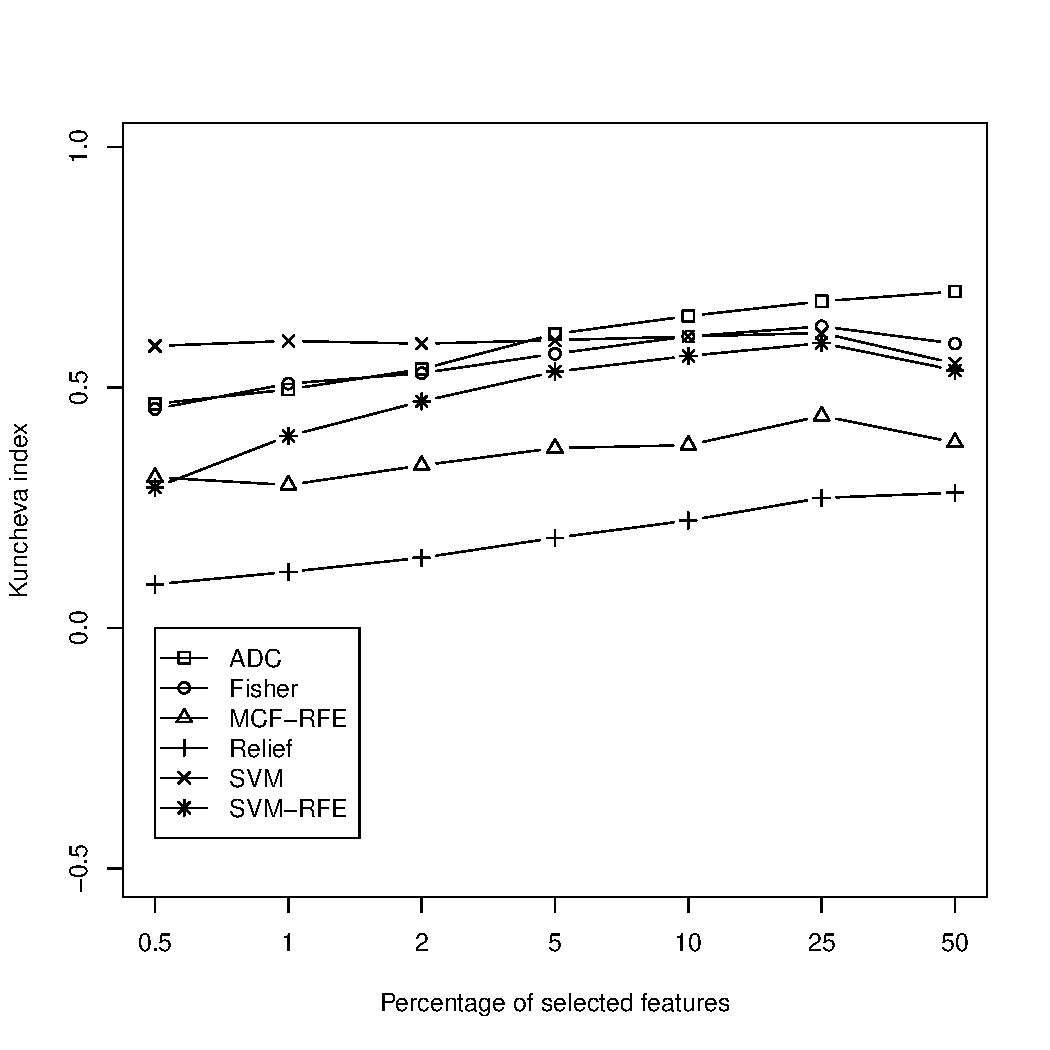
\includegraphics[width=1\textwidth]{../bachelor/images/nncns_robustness_kuncheva.pdf}
% \caption{Matų atrinkimo CNS mėginiams stabilumo grafikas pagal Kuncheva indeksą.}
% \label{fig:robk_cns}
% \end{minipage}
% \hspace{0.5cm}
% \begin{minipage}[b]{0.5\linewidth}
% \centering
% 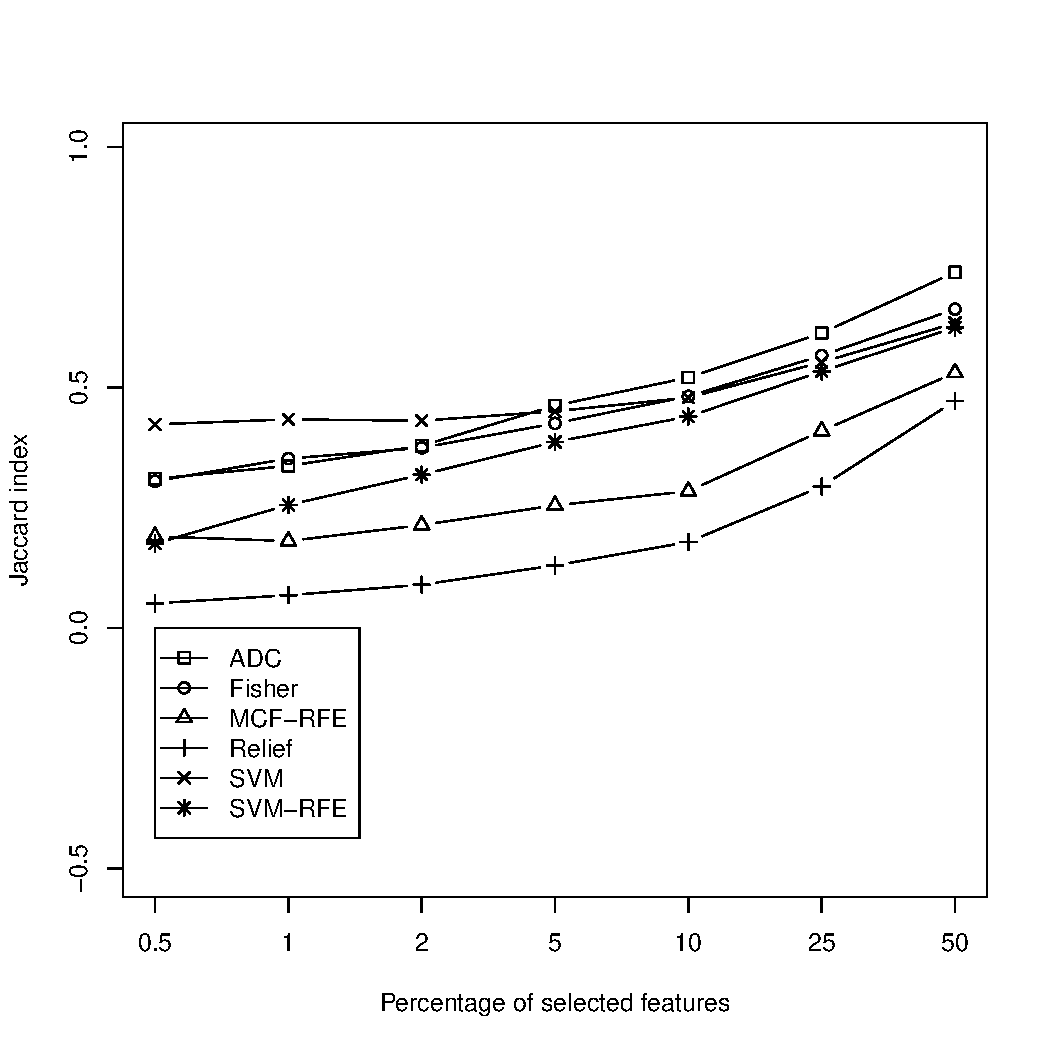
\includegraphics[width=1\textwidth]{../bachelor/images/nncns_robustness_jaccard.pdf}
% \caption{Matų atrinkimo CNS mėginiams stabilumo grafikas pagal Jaccard indeksą.}
% \label{fig:robj_cns}
% \end{minipage}
% \end{figure}
Pagal ~\ref{fig:robk_cns} pav. ir ~\ref{fig:robj_cns} pav. matome, kad centrinės nervų sistemos duomenų rinkinio matus stabiliausiai atrenka absoliučių svorių SVM matų atrinkimo metodas. Mažiausiai stabiliai matus atrenka \textit{Relief} metodas.

% \begin{figure}
% \begin{minipage}[b]{0.5\linewidth}
% \centering
% 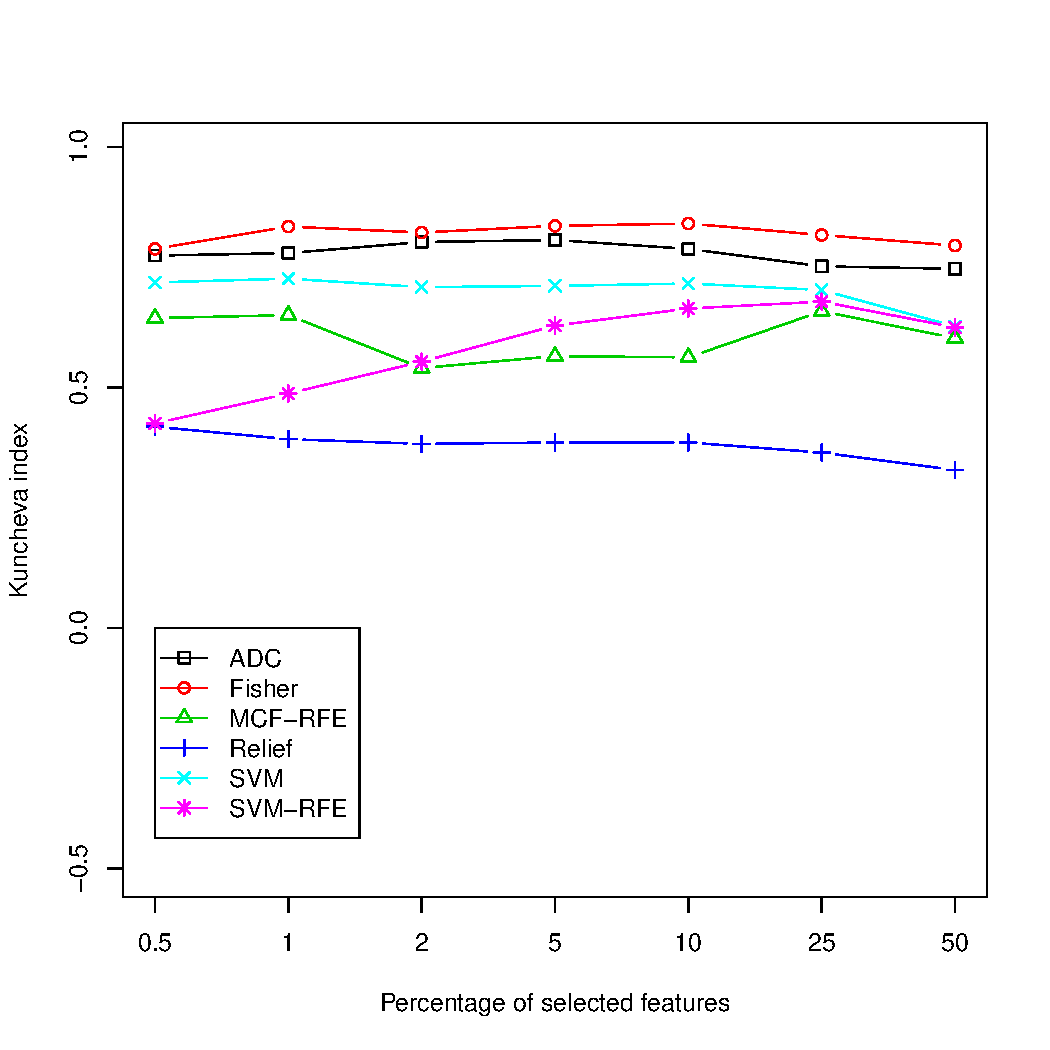
\includegraphics[width=1\textwidth]{../bachelor/images/prostate_robustness_kuncheva.pdf}
% \caption{Matų atrinkimo prostatos mėginiams stabilumo grafikas pagal Kuncheva indeksą.}
% \label{fig:robk_prostate}
% \end{minipage}
% \hspace{0.5cm}
% \begin{minipage}[b]{0.5\linewidth}
% \centering
% 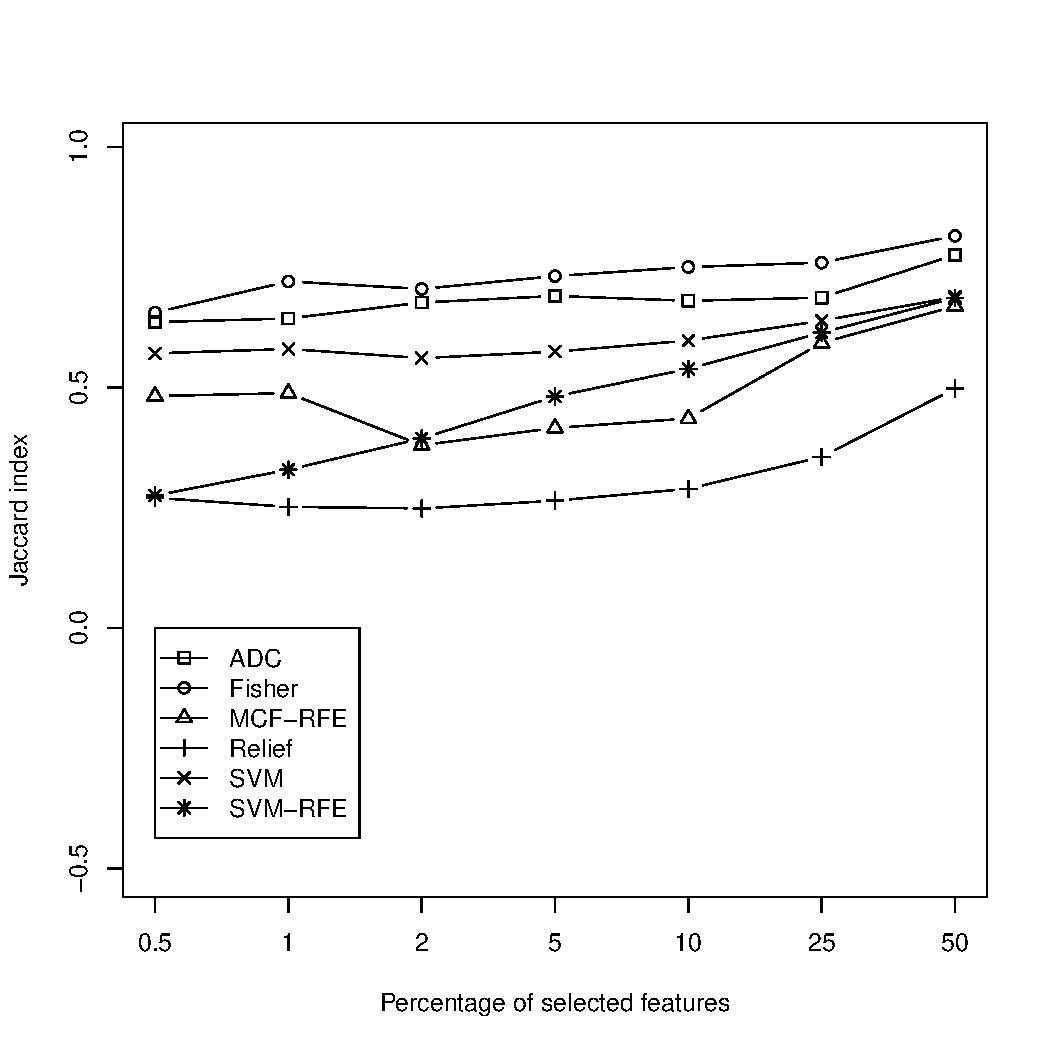
\includegraphics[width=1\textwidth]{../bachelor/images/prostate_robustness_jaccard.pdf}
% \caption{Matų atrinkimo prostatos mėginiams stabilumo grafikas pagal Jaccard indeksą.}
% \label{fig:robj_prostate}
% \end{minipage}
% \end{figure}
Pagal ~\ref{fig:robk_prostate} pav. ir ~\ref{fig:robj_prostate} pav. matome, kad prostatos duomenų rinkinio matus stabiliausiai atrenka \textit{Fisher} įvertis. Mažiausiai stabiliai matus atrenka \textit{Relief} metodas.

Apibendrindamas matų atrinkimo stabilumo matavimus galiu sakyti, kad matų atrinkimo stabilumas priklauso ne tik nuo matų atrinkimo metodo, bet ir nuo duomenų rinkinio, kurio matai yra atrinkinėjami. Lengvai klasifikuojamo prostatos duomenų rinkinio matų atrinkimo stabilumas vidutiniškai yra didesnis nei sunkiai klasifikuojamo CNS duomenų rinkinio. Eksperimentų rezultatai rodo, kad \textit{Relief} matų atrinkimo metodas yra nestabiliaus iš tirtųjų. Gana geru stabilumu pasižymi ADC metodas bei \textit{Fisher} įvertis.